\documentclass[11pt, a4paper]{article}

% --- PAQUETES ESENCIALES ---
\usepackage[spanish]{babel}
\usepackage[utf8]{inputenc}
\usepackage[T1]{fontenc}
\usepackage{lmodern}
\usepackage[margin=2.5cm]{geometry}

% --- PAQUETES PARA ESTILO ---
\usepackage{float}
\usepackage{xurl}
\usepackage{hyperref}
\usepackage{xcolor}
\usepackage{colortbl}
\usepackage{titlesec}
\usepackage{fancyhdr}
\usepackage{graphicx}
\usepackage{listings}
\usepackage{booktabs}
\usepackage{array}
\usepackage{longtable}
\usepackage{multirow}
\usepackage{caption}
\usepackage{subcaption}

% --- CONFIGURACIÓN DE COLORES Y ENLACES ---
\definecolor{primaryblue}{RGB}{0, 83, 156}
\definecolor{linkcolor}{RGB}{0, 102, 204}
\definecolor{codegray}{rgb}{0.5,0.5,0.5}
\definecolor{backcolour}{rgb}{0.95,0.95,0.95}

\hypersetup{
    colorlinks=true,
    linkcolor=primaryblue,
    urlcolor=linkcolor,
    pdftitle={},
    pdfauthor={Ángel Manuel Pereira Rodríguez}
}

% --- ESTILO DE TÍTULOS ---
\titleformat{\section}
{\color{primaryblue}\normalfont\Large\bfseries}
{\thesection}{1em}{}

\titleformat{\subsection}
{\color{primaryblue}\normalfont\large\bfseries}
{\thesubsection}{1em}{}

\titleformat{\subsubsection}
{\color{primaryblue}\normalfont\normalsize\bfseries}
{\thesubsubsection}{1em}{}

% --- CABECERA Y PIE DE PÁGINA ---
\pagestyle{fancy}
\fancyhf{}
\rhead{\small\textcolor{gray}{}}
\lhead{\small\textcolor{gray}{\today}}
\cfoot{\thepage}
\renewcommand{\headrulewidth}{0.4pt}

% --- CONFIGURACIÓN DE LISTINGS ---
\lstdefinestyle{mystyle}{
    backgroundcolor=\color{backcolour},
    commentstyle=\color{green!50!black},
    keywordstyle=\color{blue},
    numberstyle=\tiny\color{codegray},
    stringstyle=\color{red},
    basicstyle=\ttfamily\footnotesize,
    breakatwhitespace=false,
    breaklines=true,
    captionpos=b,
    keepspaces=true,
    numbers=left,
    numbersep=5pt,
    showspaces=false,
    showstringspaces=false,
    showtabs=false,
    tabsize=2
}

\lstset{style=mystyle}

% --- TÍTULO DEL DOCUMENTO ---
\title{Memoria T\'ecnica\\OCR Layout + Multi-OCR + Evaluaci\'on con Ground Truth}
\author{Ángel Manuel Pereira Rodríguez}
\date{\today}

\begin{document}

\maketitle

\begin{abstract}
Esta memoria t\'ecnica describe el desarrollo completo del proyecto de visi\'on artificial
orientado a documentos hist\'oricos escaneados. El sistema combina varios m\'etodos de
detecci\'on de layout, varios motores OCR y un proceso de evaluaci\'on con ground truth
para medir calidad real de extracci\'on. A lo largo del proyecto se implement\'o un pipeline
reproducible que cubre detecci\'on de regiones de texto, b\'usqueda sistem\'atica de
configuraciones, ranking heur\'istico, validaci\'on OCR multi-motor y comparaci\'on final
mediante CER, WER y m\'etricas de orden de lectura. La memoria resume la arquitectura,
las im\'agenes utilizadas, los resultados obtenidos y el procedimiento de instalaci\'on y uso.
\end{abstract}

\tableofcontents
\listoffigures
\listoftables
\clearpage

\section{Introducci\'on}

El objetivo del proyecto ha sido construir un sistema robusto para analizar documentos
impresos antiguos con OCR, teniendo en cuenta que el principal cuello de botella no es solo
el motor de reconocimiento, sino tambi\'en la calidad del layout previo. En este tipo de
material aparecen varios problemas combinados:

\begin{itemize}
    \item P\'aginas dobles o composiciones con varias columnas,
    \item Anuncios y zonas decorativas mezcladas con texto,
    \item Escaneos envejecidos, pliegues, sombras y baja uniformidad,
    \item Necesidad de mantener un orden de lectura razonable.
\end{itemize}

Para resolverlo, el proyecto no se limit\'o a aplicar OCR directamente sobre la imagen
completa. En su lugar, se dise\~n\'o un pipeline por fases:

\begin{enumerate}
    \item Detecci\'on de layout por varios m\'etodos,
    \item Experimentaci\'on sistem\'atica de configuraciones,
    \item Ranking de configuraciones de detecci\'on,
    \item Validaci\'on OCR con varios motores sobre las mismas regiones,
    \item Comparaci\'on final frente a ground truth.
\end{enumerate}

Este enfoque permite separar con claridad dos tipos de error:

\begin{itemize}
    \item Errores de segmentaci\'on del documento,
    \item Errores de reconocimiento del texto.
\end{itemize}

\section{Objetivos del proyecto}

Los objetivos principales han sido los siguientes:

\begin{itemize}
    \item Detectar regiones de texto de forma fiable en documentos hist\'oricos escaneados,
    \item Comparar distintos m\'etodos de layout en un mismo conjunto de im\'agenes,
    \item Medir el comportamiento de varios motores OCR bajo condiciones equivalentes,
    \item Crear un ground truth de referencia para evaluaci\'on objetiva,
    \item Dejar un sistema instalable, reproducible y extensible.
\end{itemize}

La unidad real de evaluaci\'on del sistema es:

\begin{center}
\texttt{configuraci\'on\_de\_layout x motor\_ocr x imagen}
\end{center}

\section{Arquitectura general del sistema}

El repositorio est\'a organizado alrededor de varios scripts especializados. Los m\'as
importantes son:

\begin{itemize}
    \item \texttt{detect\_columns.py}: Detecci\'on de layout por m\'ultiples m\'etodos.
    \item \texttt{post\_processing.py}: NMS, merge y limpieza de cajas.
    \item \texttt{experiment\_models.py}: Grid search sobre configuraciones de layout.
    \item \texttt{analyze\_experiments.py}: Ranking agregado de configuraciones.
    \item \texttt{validate\_ocr.py}: Validaci\'on multi-motor OCR.
    \item \texttt{compare\_validation\_vs\_ground\_truth.py}: Comparaci\'on con ground truth.
    \item Scripts OCR individuales para pruebas por motor y depuraci\'on comparativa.
\end{itemize}

Los m\'etodos de layout implementados son:

\begin{itemize}
    \item \texttt{opencv}: Enfoque heur\'istico, muy r\'apido, sin modelos profundos.
    \item \texttt{doclayout}: DocLayout-YOLO basado en YOLOv10 y DocStructBench.
    \item \texttt{yolo11}: Modelo YOLO11 fine-tuned sobre DocLayNet.
    \item \texttt{paddleocr}: Detector de layout de PaddleOCR PP-StructureV3.
    \item \texttt{docling}: Detector de layout de IBM Docling.
\end{itemize}

Los motores OCR comparados son:

\begin{itemize}
    \item EasyOCR,
    \item Tesseract,
    \item PaddleOCR,
    \item DeepSeek-OCR.
\end{itemize}

\section{Im\'agenes utilizadas}

El conjunto de trabajo utilizado en el proyecto est\'a compuesto por 18 im\'agenes en la
carpeta \texttt{imgs/}, nombradas de \texttt{popurri01.jpg} a \texttt{popurri18.jpg}. Todas
ellas pertenecen a material hist\'orico escaneado relacionado con agrupaciones, anuncios,
popurr\'is y documentos de carnaval, con gran variedad de dise\~nos y distribuciones.

Este conjunto resulta \'util porque mezcla casos relativamente limpios con otros mucho m\'as
dif\'iciles, incluyendo:

\begin{itemize}
    \item P\'aginas simples con una sola masa textual,
    \item Dobles p\'aginas con varias columnas,
    \item Anuncios tipogr\'aficos decorativos,
    \item Documentos con ilustraciones o botellas,
    \item Fichas biogr\'aficas con texto continuo de alto contraste.
\end{itemize}

\begin{table}[H]
\centering
\caption{Resumen del conjunto de im\'agenes utilizado}
\begin{tabular}{p{3.3cm} p{9.5cm}}
\toprule
\textbf{Elemento} & \textbf{Descripci\'on} \\
\midrule
Conjunto principal & 18 im\'agenes \texttt{popurri01.jpg} a \texttt{popurri18.jpg} \\
Tipo de fuente & Escaneos hist\'oricos de documentos impresos \\
Variabilidad visual & Alta: columnas, dobles p\'aginas, anuncios, tipograf\'ias decorativas y fondos envejecidos \\
Uso dentro del proyecto & Detecci\'on, grid search, ranking, validaci\'on OCR y evaluaci\'on con ground truth \\
Ground truth & Disponible para las 18 im\'agenes en el archivo \texttt{ground\_truth/ocr\_ground\_truth.json} \\
\bottomrule
\end{tabular}
\end{table}

\begin{figure}[H]
    \centering
    \begin{subfigure}[b]{0.31\textwidth}
        \centering
        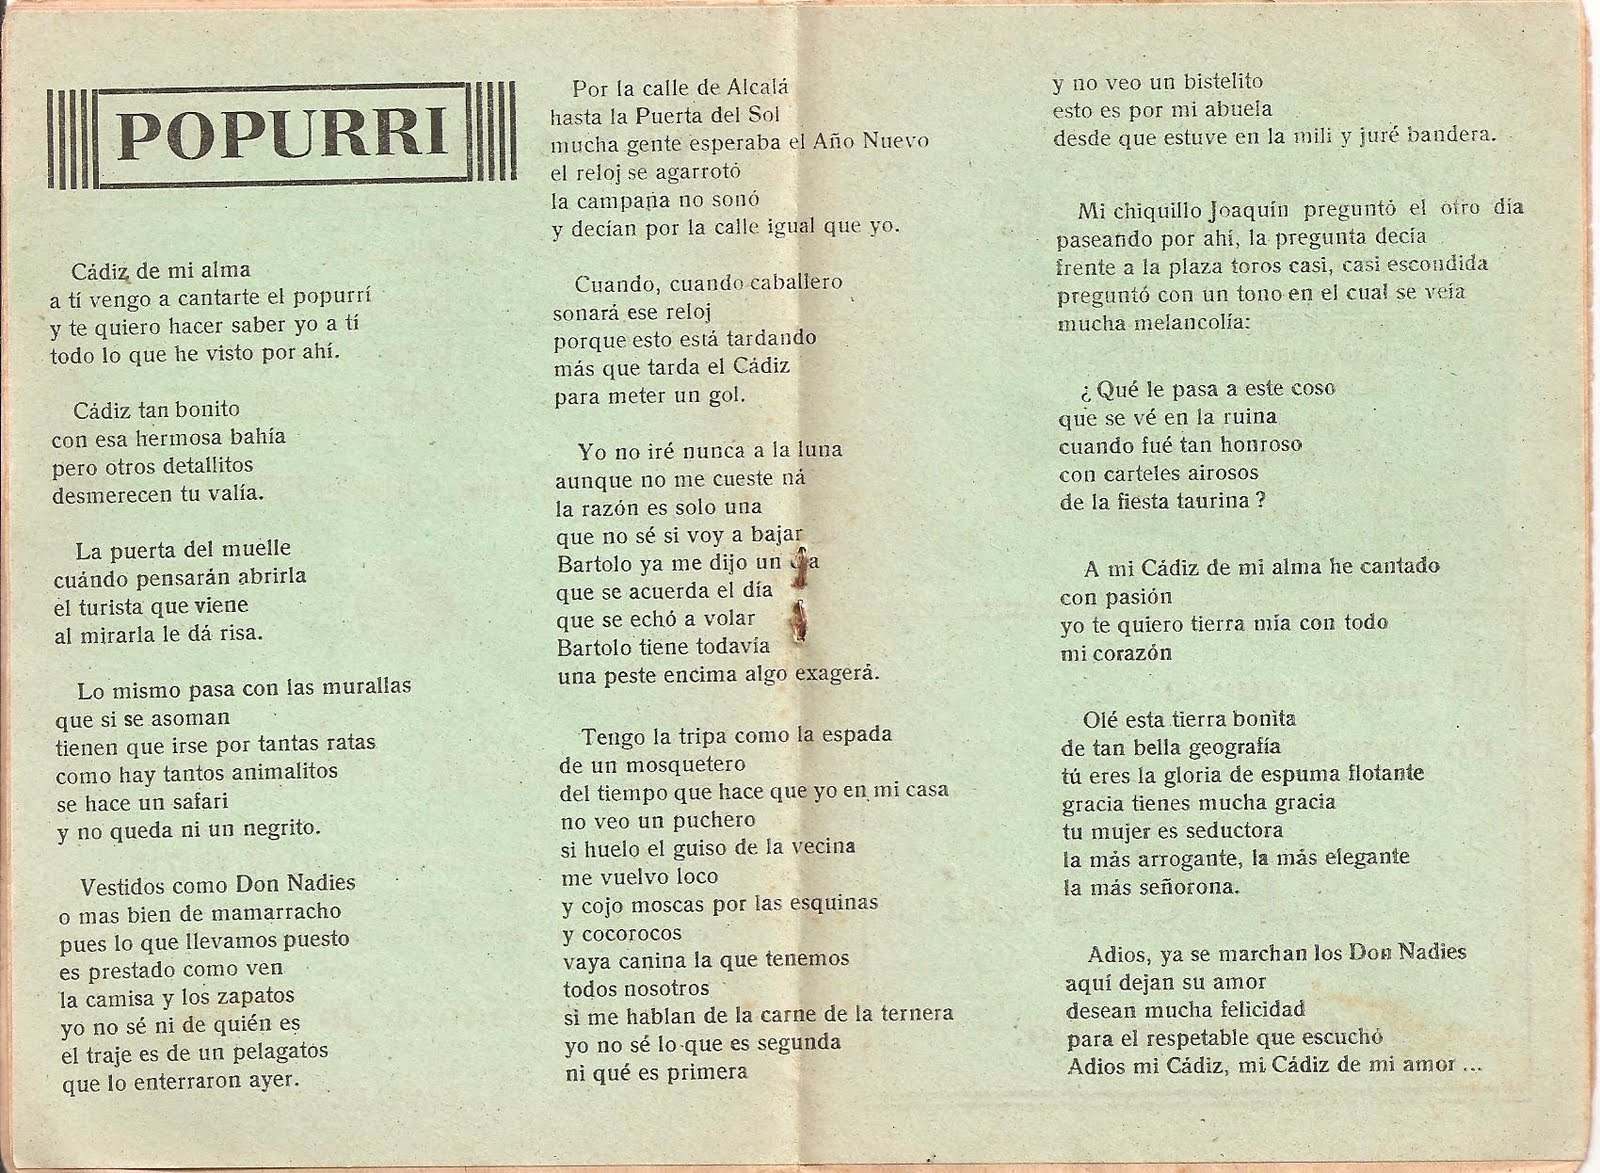
\includegraphics[width=\textwidth,height=4cm,keepaspectratio]{imgs/popurri01.jpg}
        \caption{popurri01}
    \end{subfigure}
    \hfill
    \begin{subfigure}[b]{0.31\textwidth}
        \centering
        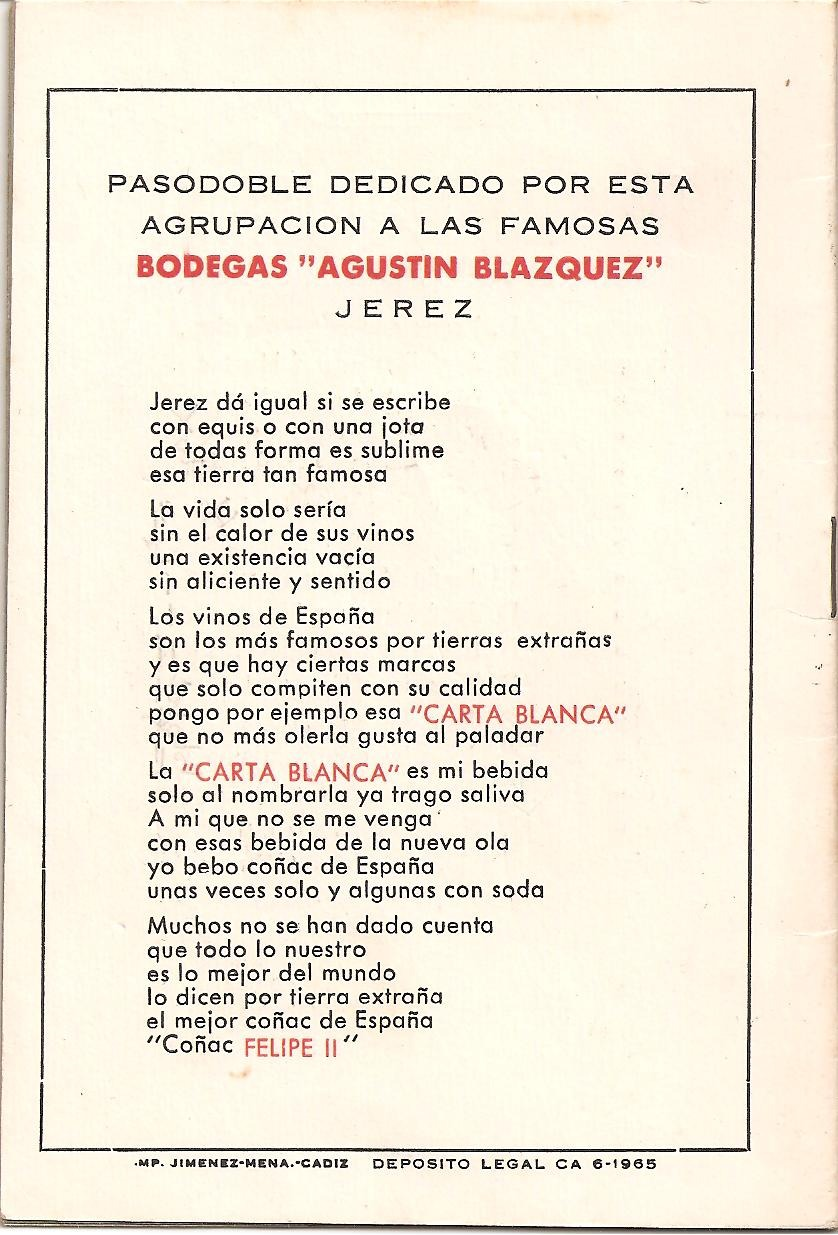
\includegraphics[width=\textwidth,height=4cm,keepaspectratio]{imgs/popurri02.jpg}
        \caption{popurri02}
    \end{subfigure}
    \hfill
    \begin{subfigure}[b]{0.31\textwidth}
        \centering
        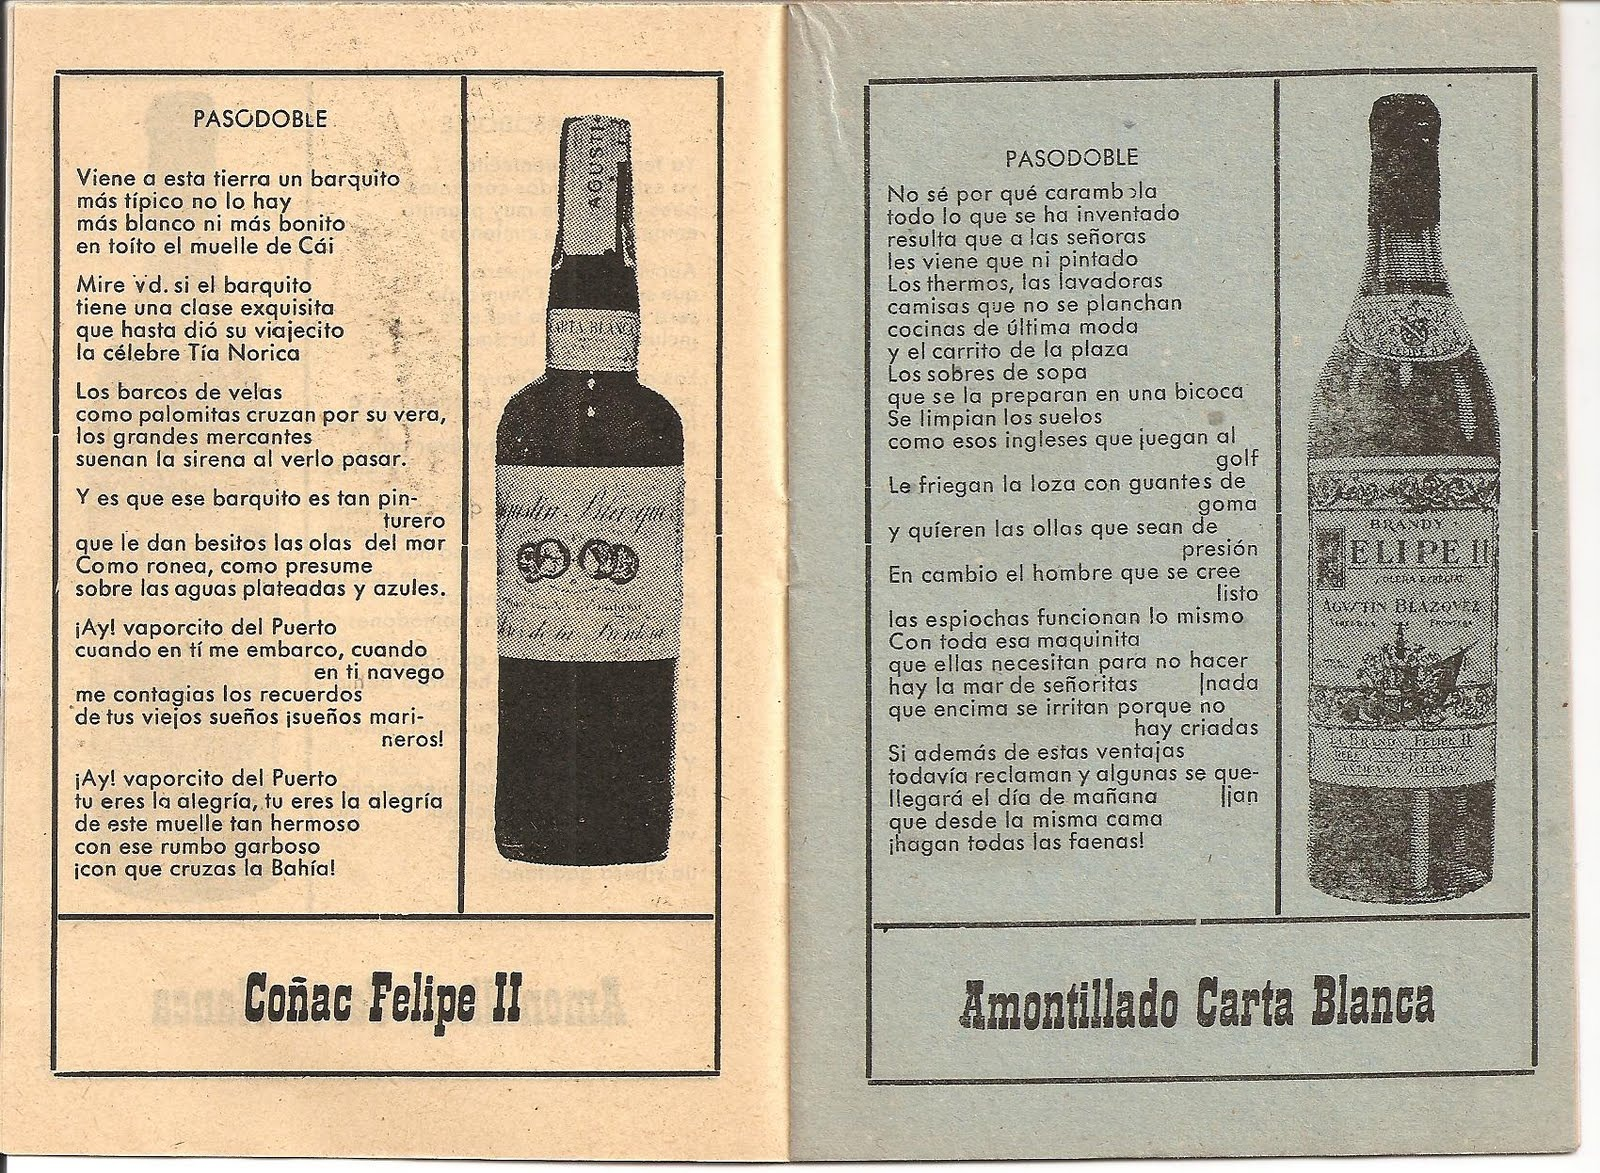
\includegraphics[width=\textwidth,height=4cm,keepaspectratio]{imgs/popurri03.jpg}
        \caption{popurri03}
    \end{subfigure}

    \vspace{0.4cm}

    \begin{subfigure}[b]{0.31\textwidth}
        \centering
        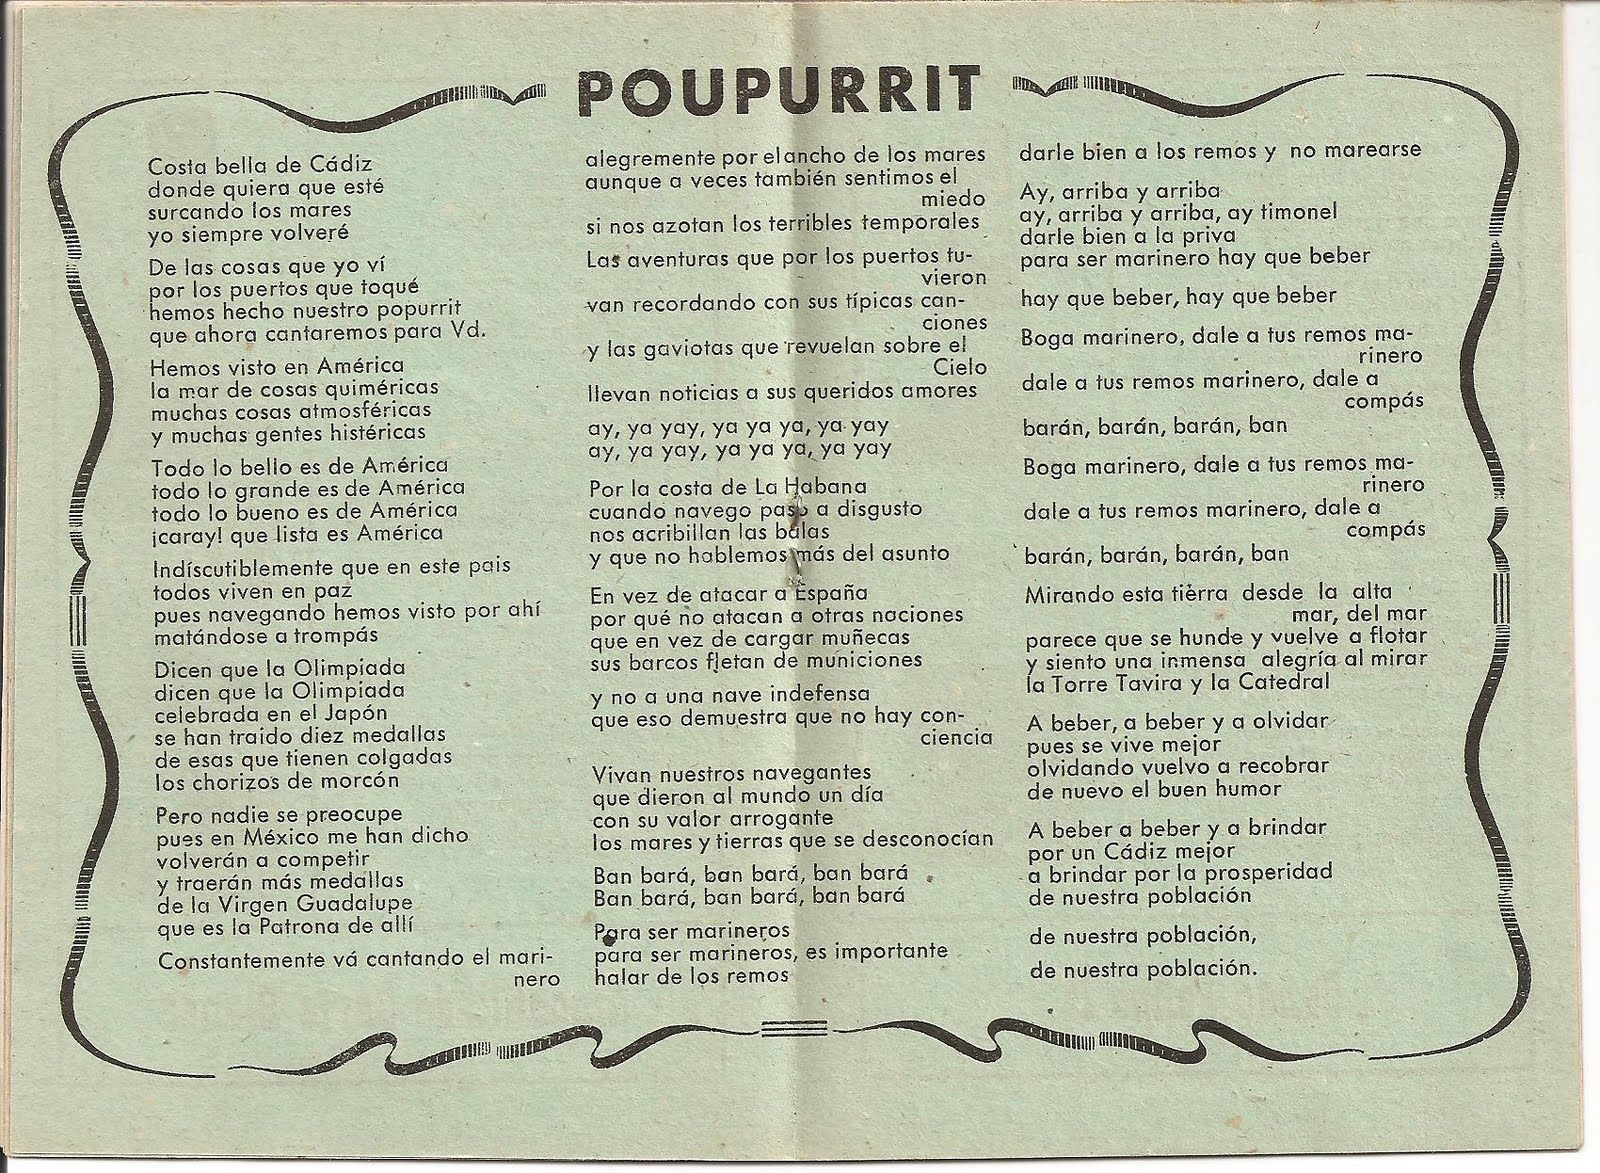
\includegraphics[width=\textwidth,height=4cm,keepaspectratio]{imgs/popurri04.jpg}
        \caption{popurri04}
    \end{subfigure}
    \hfill
    \begin{subfigure}[b]{0.31\textwidth}
        \centering
        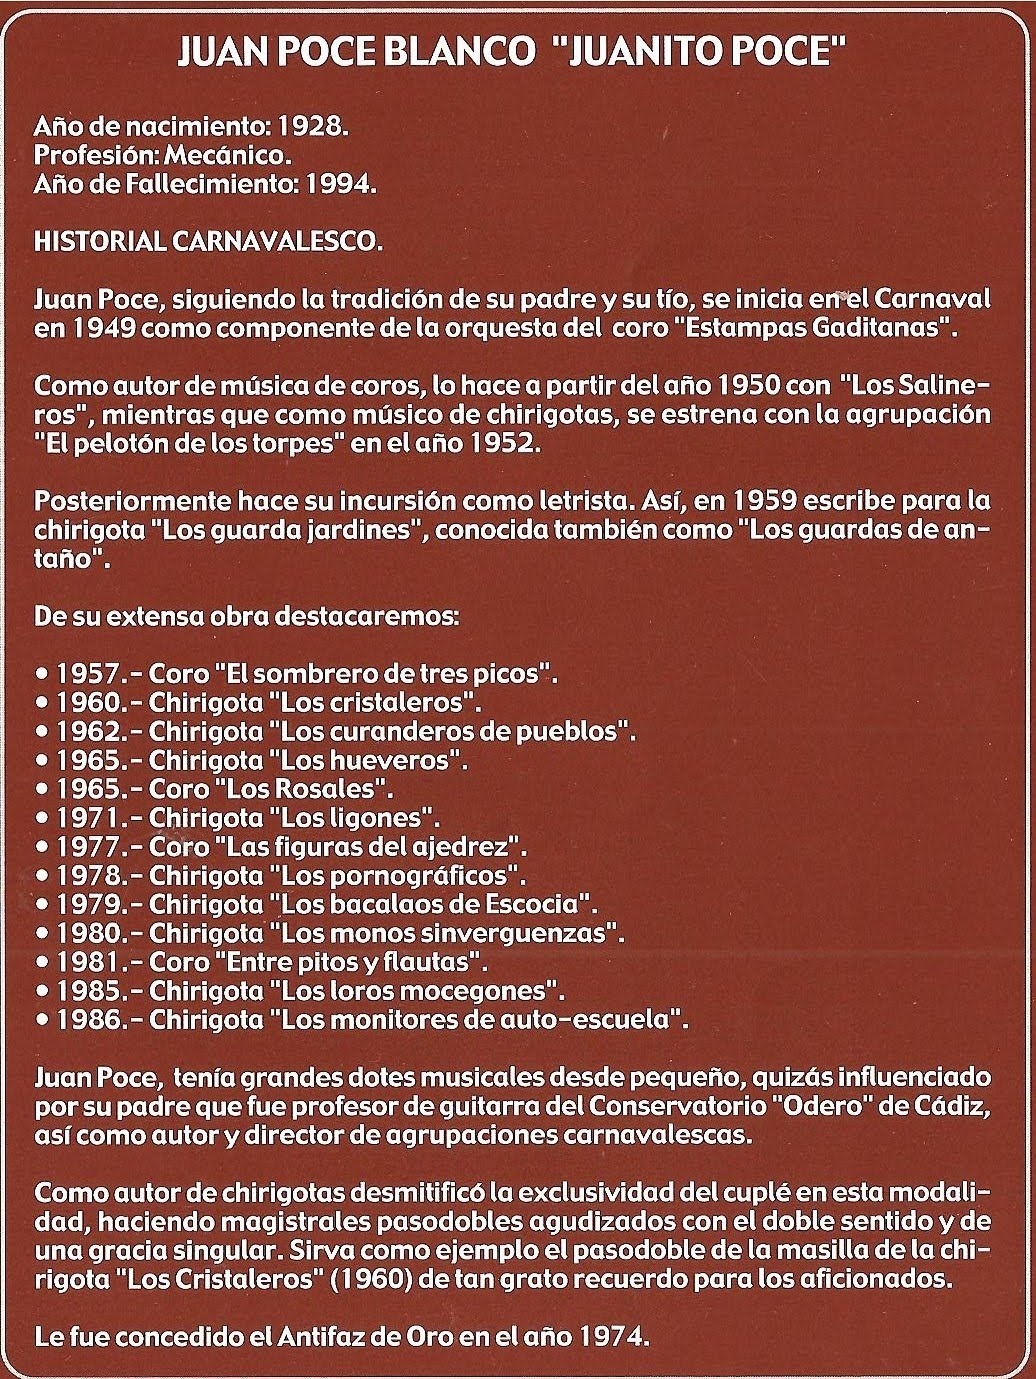
\includegraphics[width=\textwidth,height=4cm,keepaspectratio]{imgs/popurri05.jpg}
        \caption{popurri05}
    \end{subfigure}
    \hfill
    \begin{subfigure}[b]{0.31\textwidth}
        \centering
        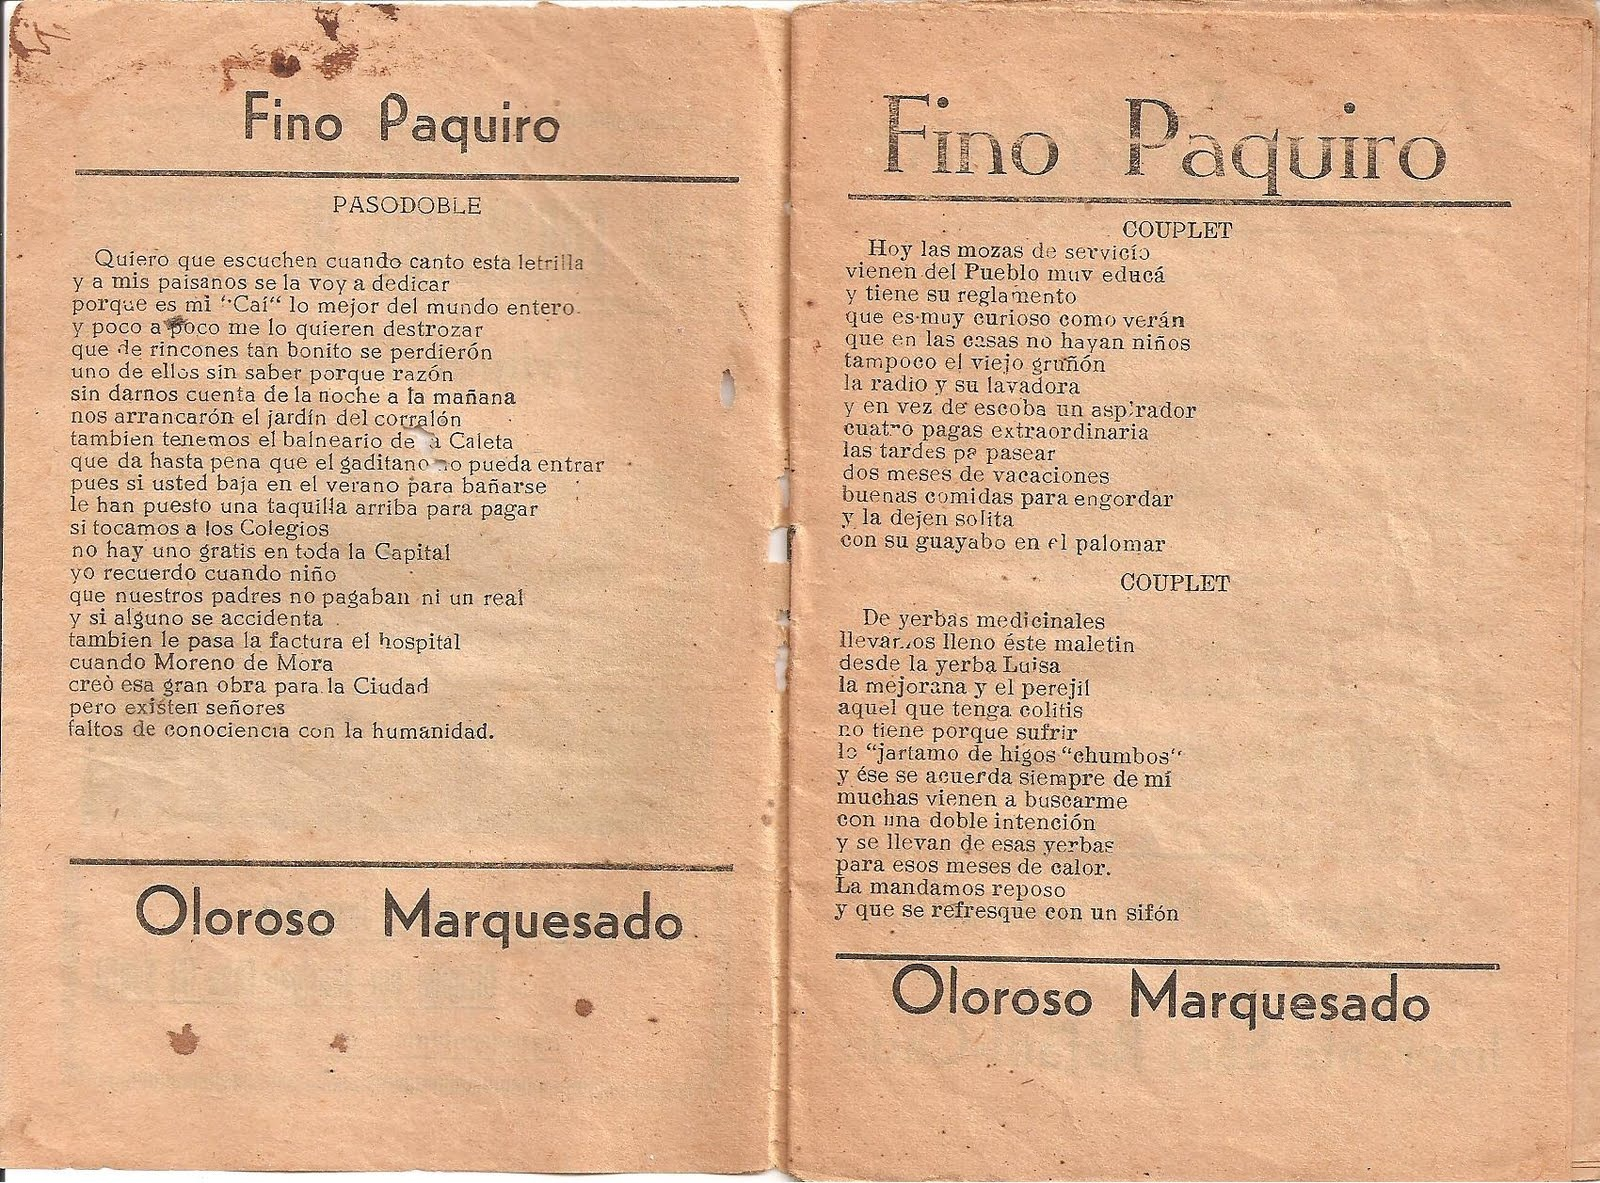
\includegraphics[width=\textwidth,height=4cm,keepaspectratio]{imgs/popurri06.jpg}
        \caption{popurri06}
    \end{subfigure}
    \caption{Galer\'ia del dataset, bloque 1 de 3.}
\end{figure}

\begin{figure}[H]
    \centering
    \begin{subfigure}[b]{0.31\textwidth}
        \centering
        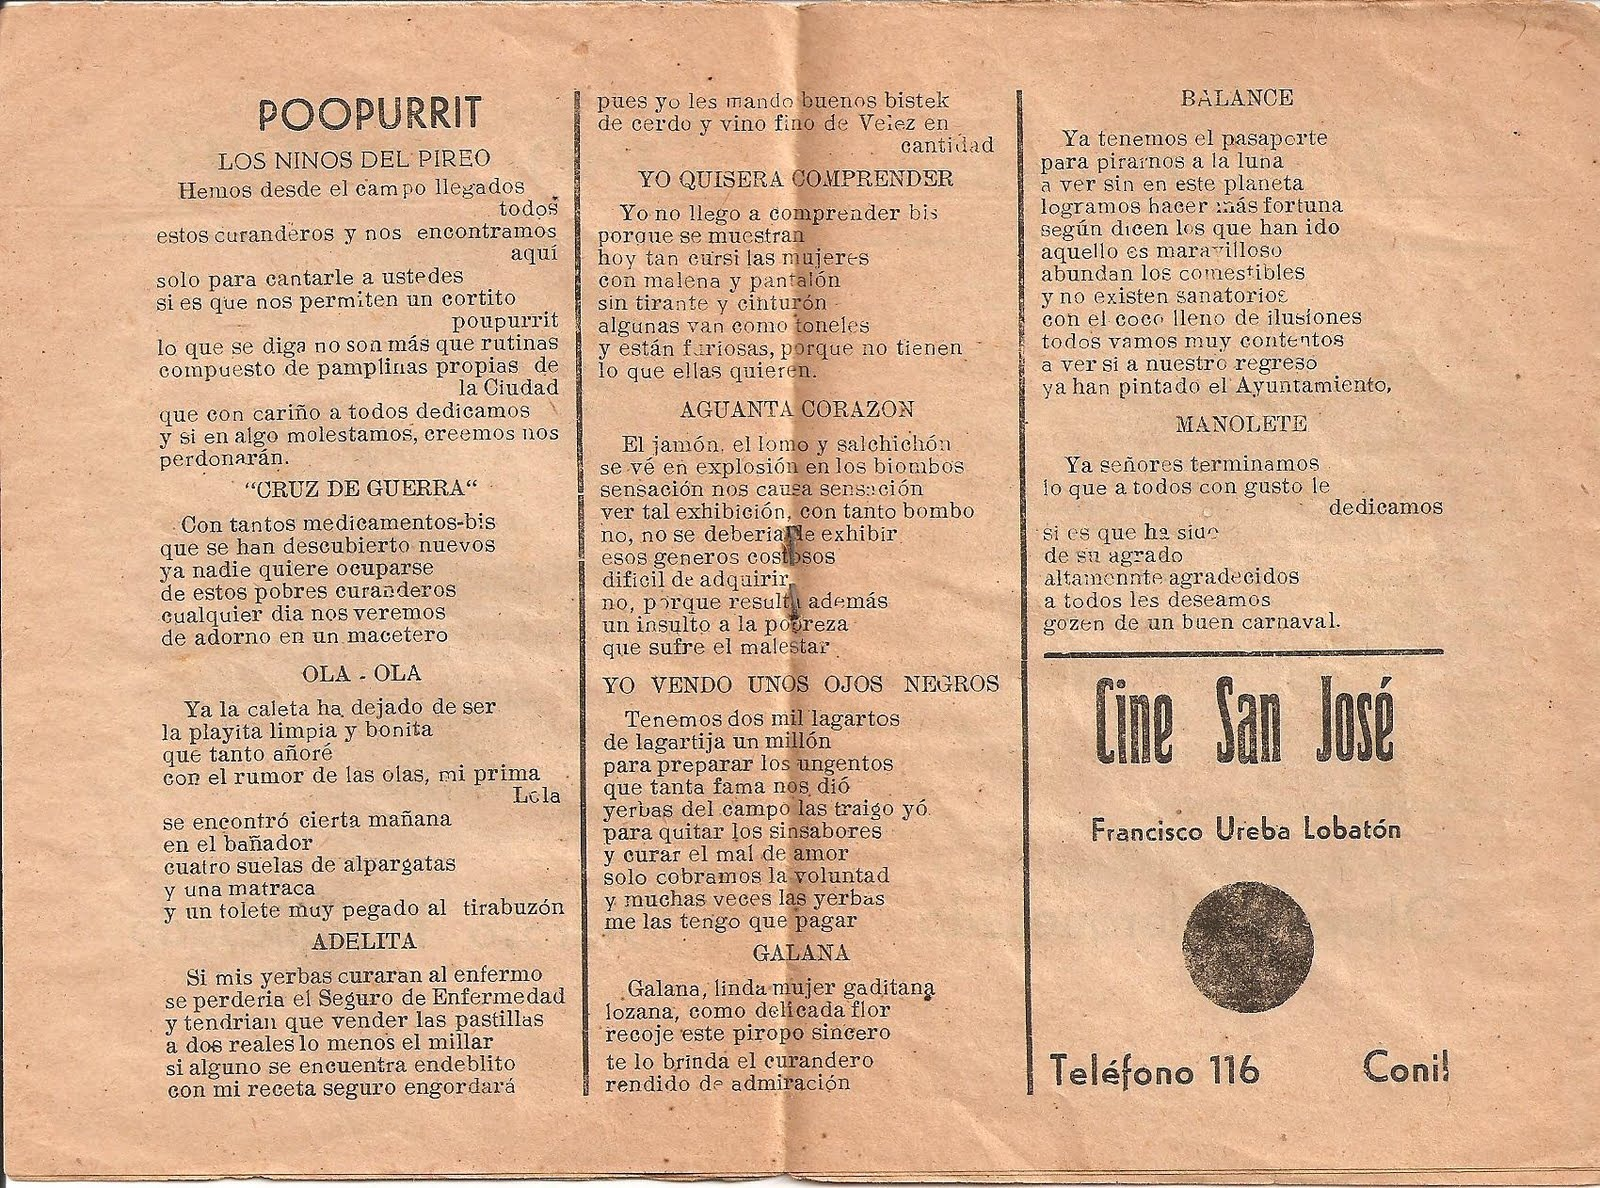
\includegraphics[width=\textwidth,height=4cm,keepaspectratio]{imgs/popurri07.jpg}
        \caption{popurri07}
    \end{subfigure}
    \hfill
    \begin{subfigure}[b]{0.31\textwidth}
        \centering
        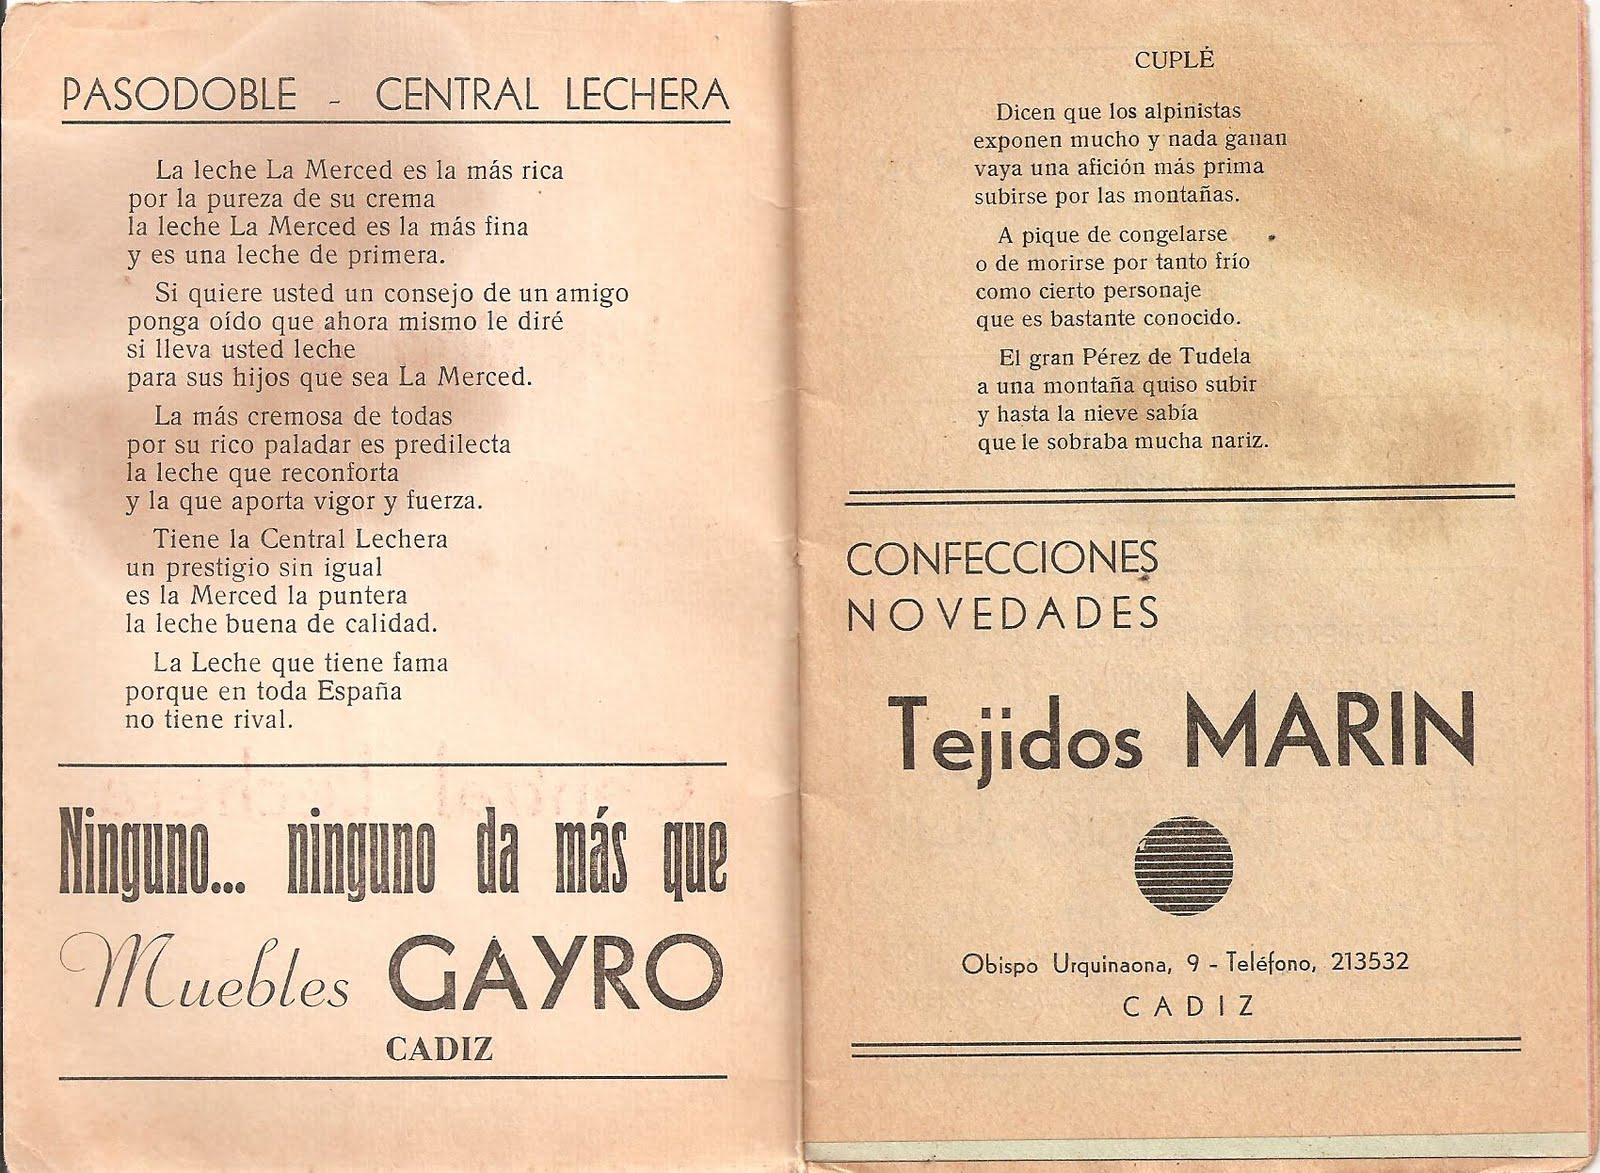
\includegraphics[width=\textwidth,height=4cm,keepaspectratio]{imgs/popurri08.jpg}
        \caption{popurri08}
    \end{subfigure}
    \hfill
    \begin{subfigure}[b]{0.31\textwidth}
        \centering
        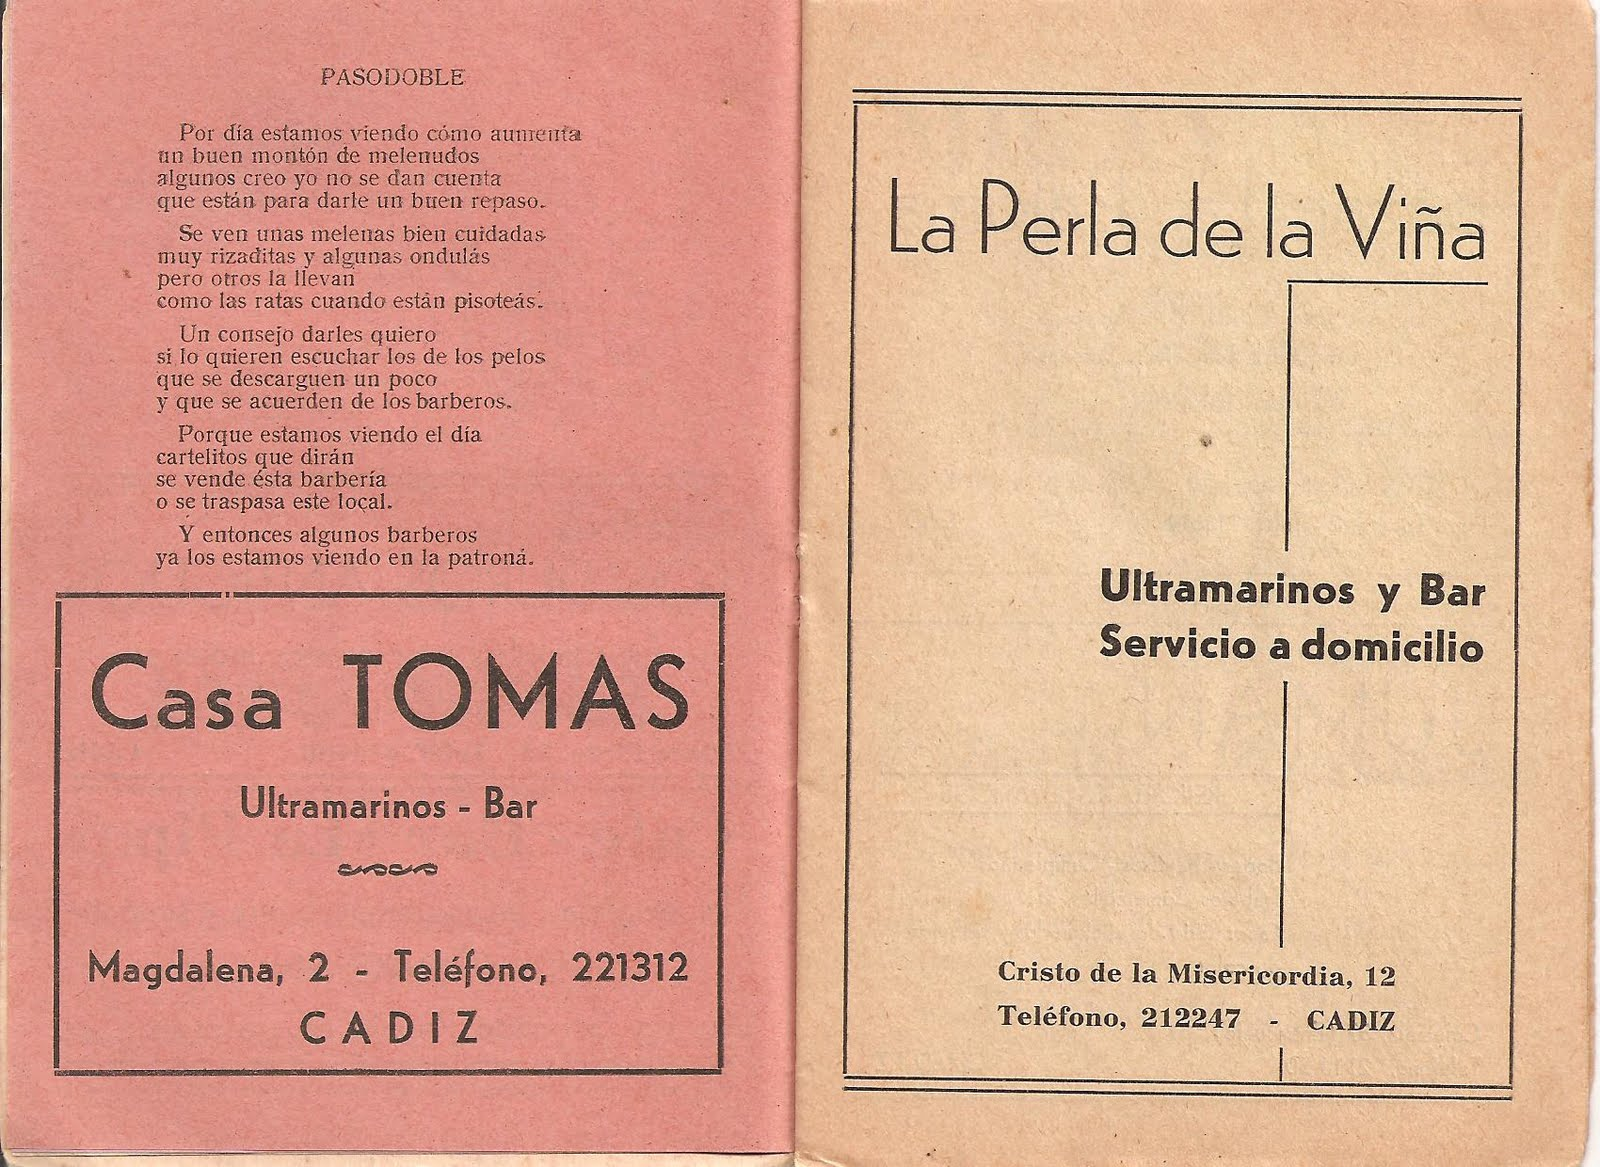
\includegraphics[width=\textwidth,height=4cm,keepaspectratio]{imgs/popurri09.jpg}
        \caption{popurri09}
    \end{subfigure}

    \vspace{0.4cm}

    \begin{subfigure}[b]{0.31\textwidth}
        \centering
        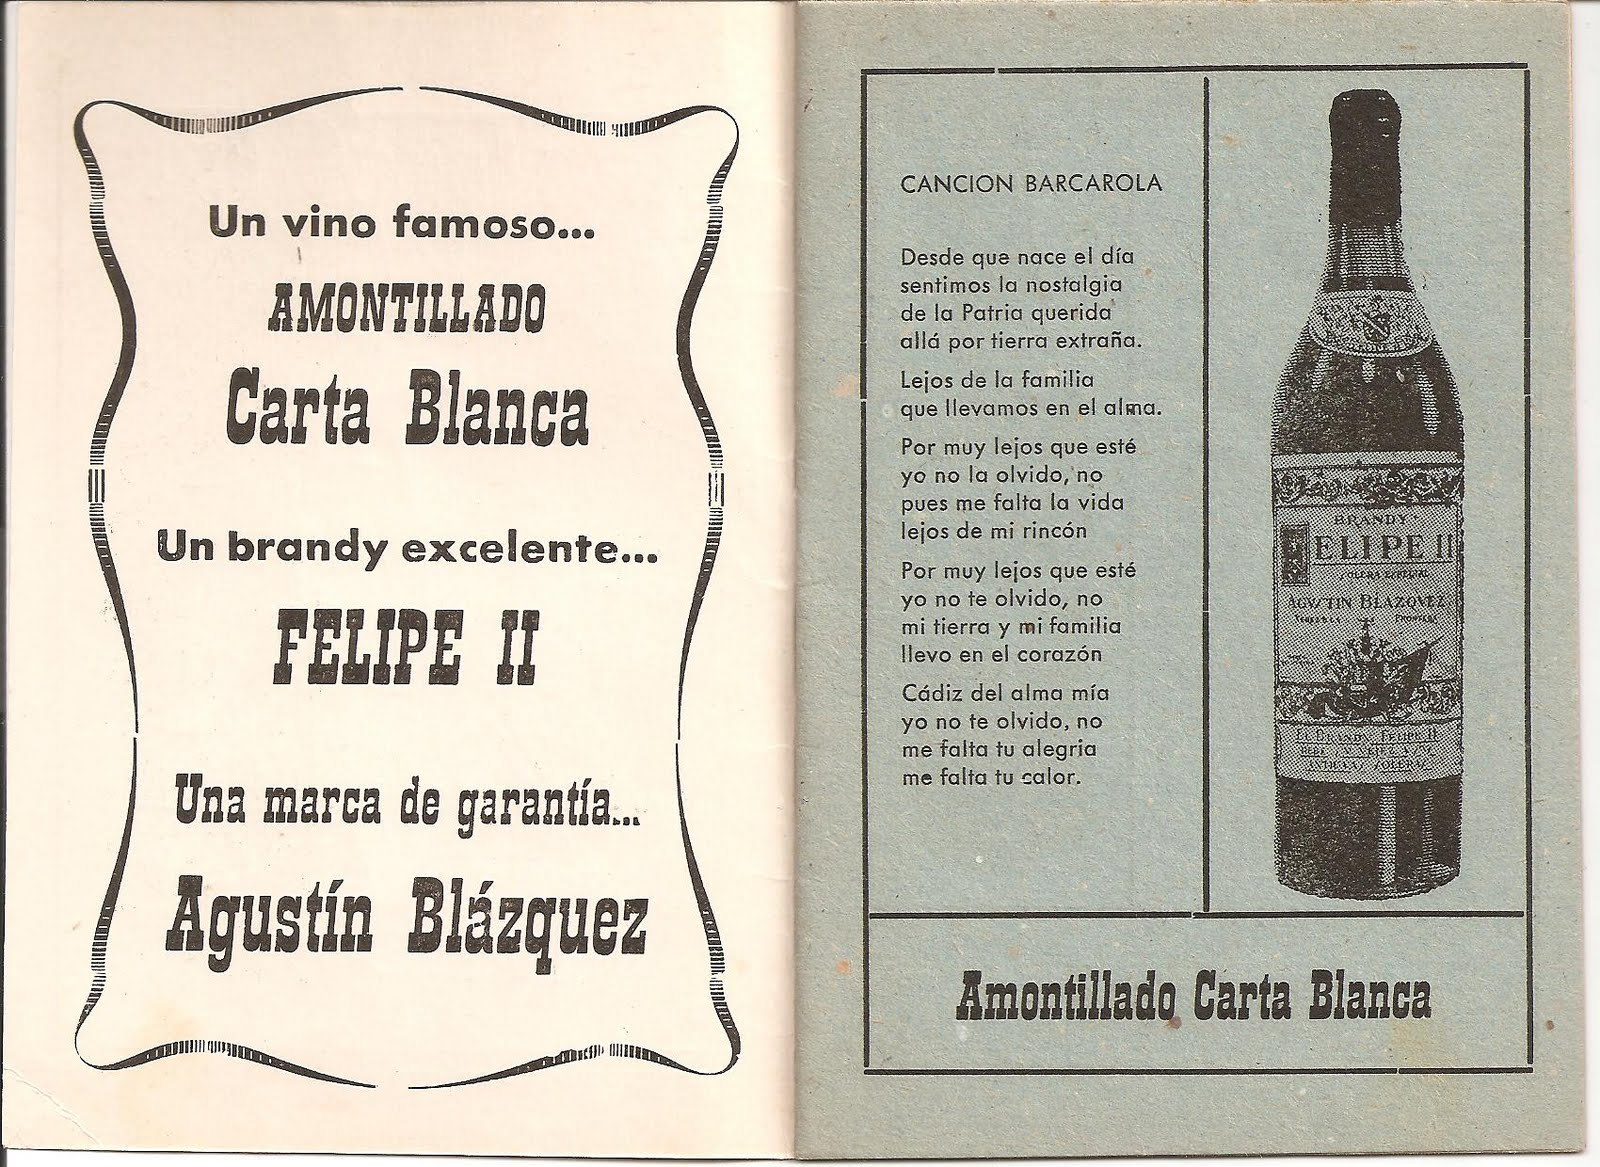
\includegraphics[width=\textwidth,height=4cm,keepaspectratio]{imgs/popurri10.jpg}
        \caption{popurri10}
    \end{subfigure}
    \hfill
    \begin{subfigure}[b]{0.31\textwidth}
        \centering
        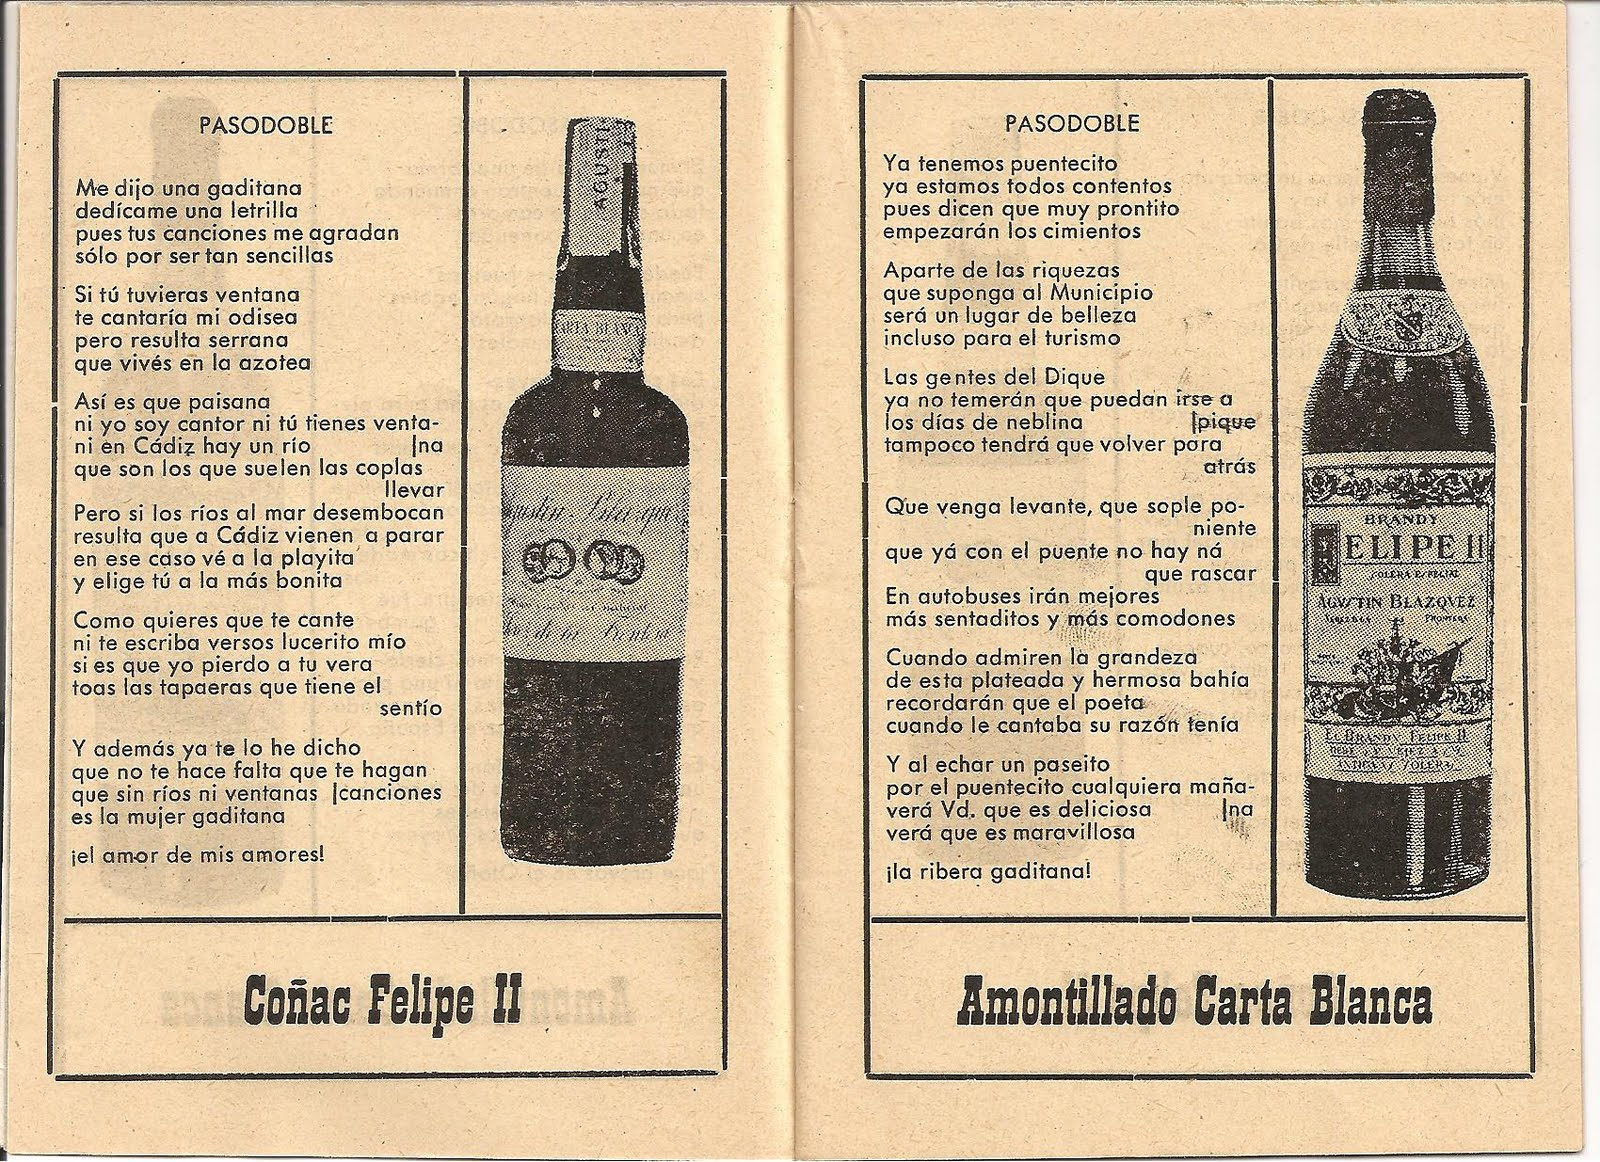
\includegraphics[width=\textwidth,height=4cm,keepaspectratio]{imgs/popurri11.jpg}
        \caption{popurri11}
    \end{subfigure}
    \hfill
    \begin{subfigure}[b]{0.31\textwidth}
        \centering
        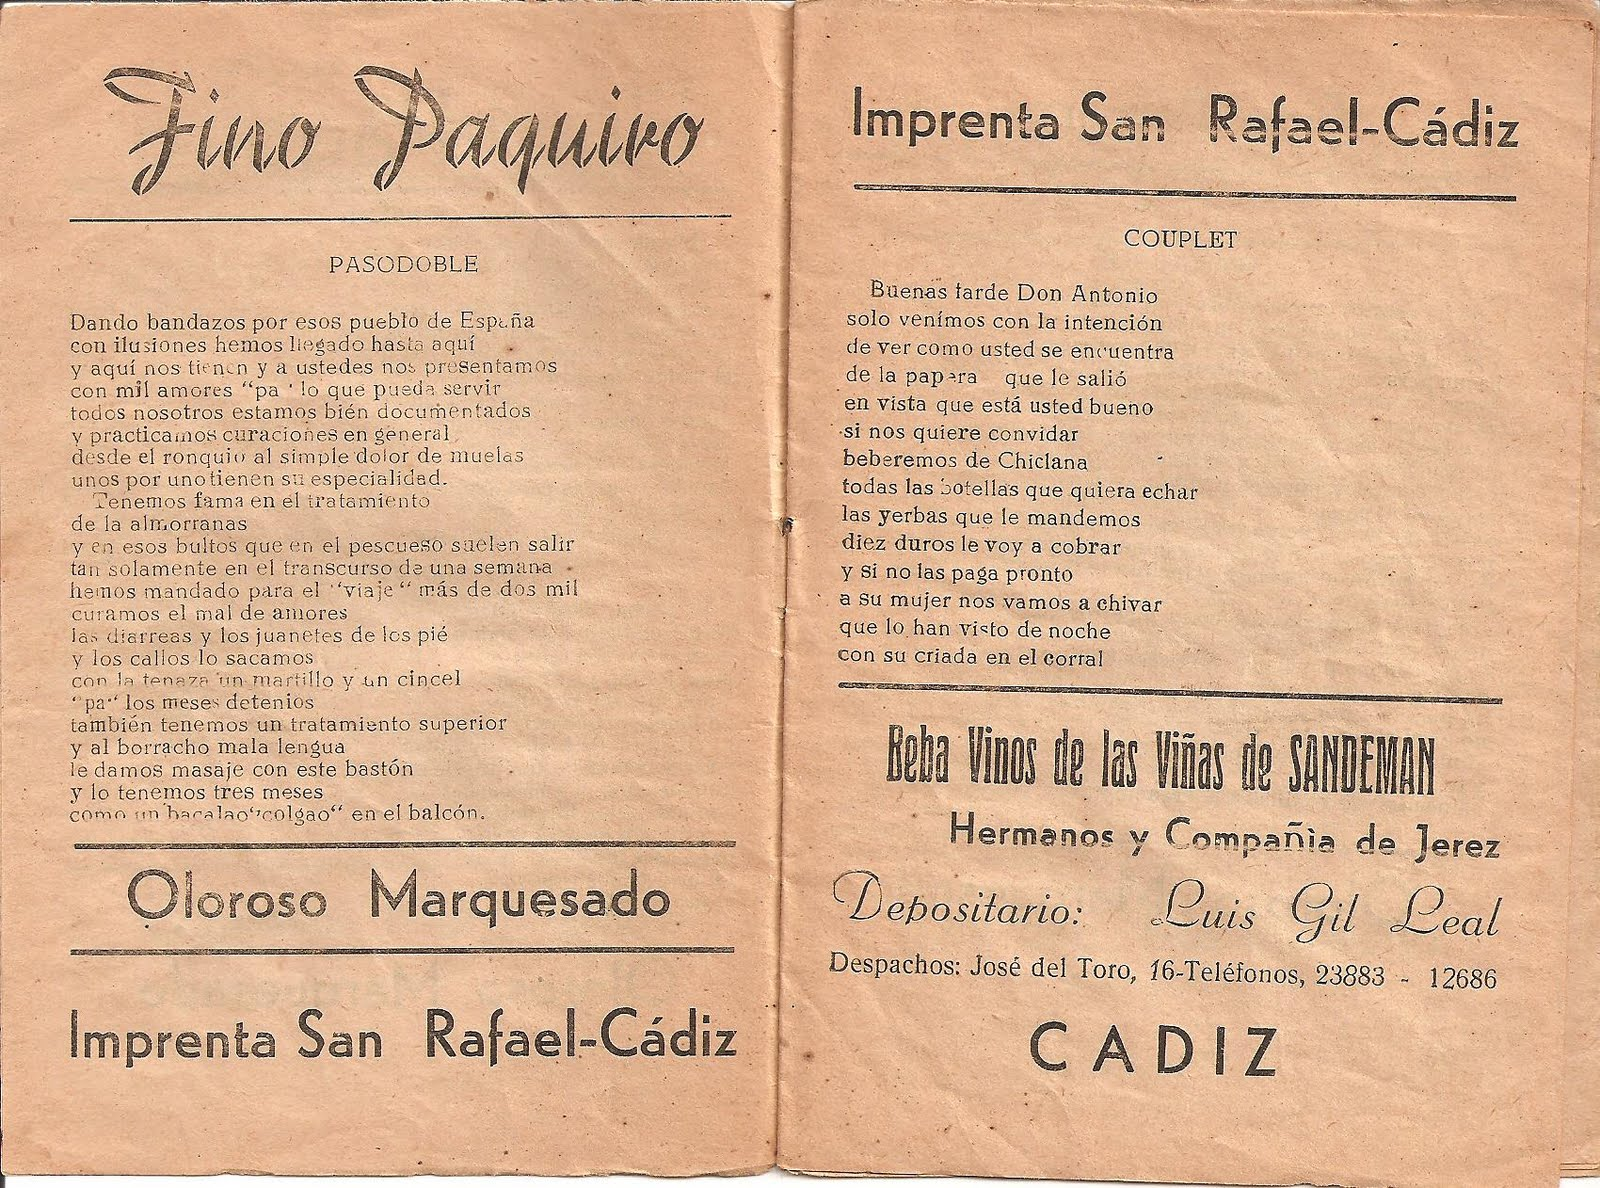
\includegraphics[width=\textwidth,height=4cm,keepaspectratio]{imgs/popurri12.jpg}
        \caption{popurri12}
    \end{subfigure}
    \caption{Galer\'ia del dataset, bloque 2 de 3.}
\end{figure}

\begin{figure}[H]
    \centering
    \begin{subfigure}[b]{0.31\textwidth}
        \centering
        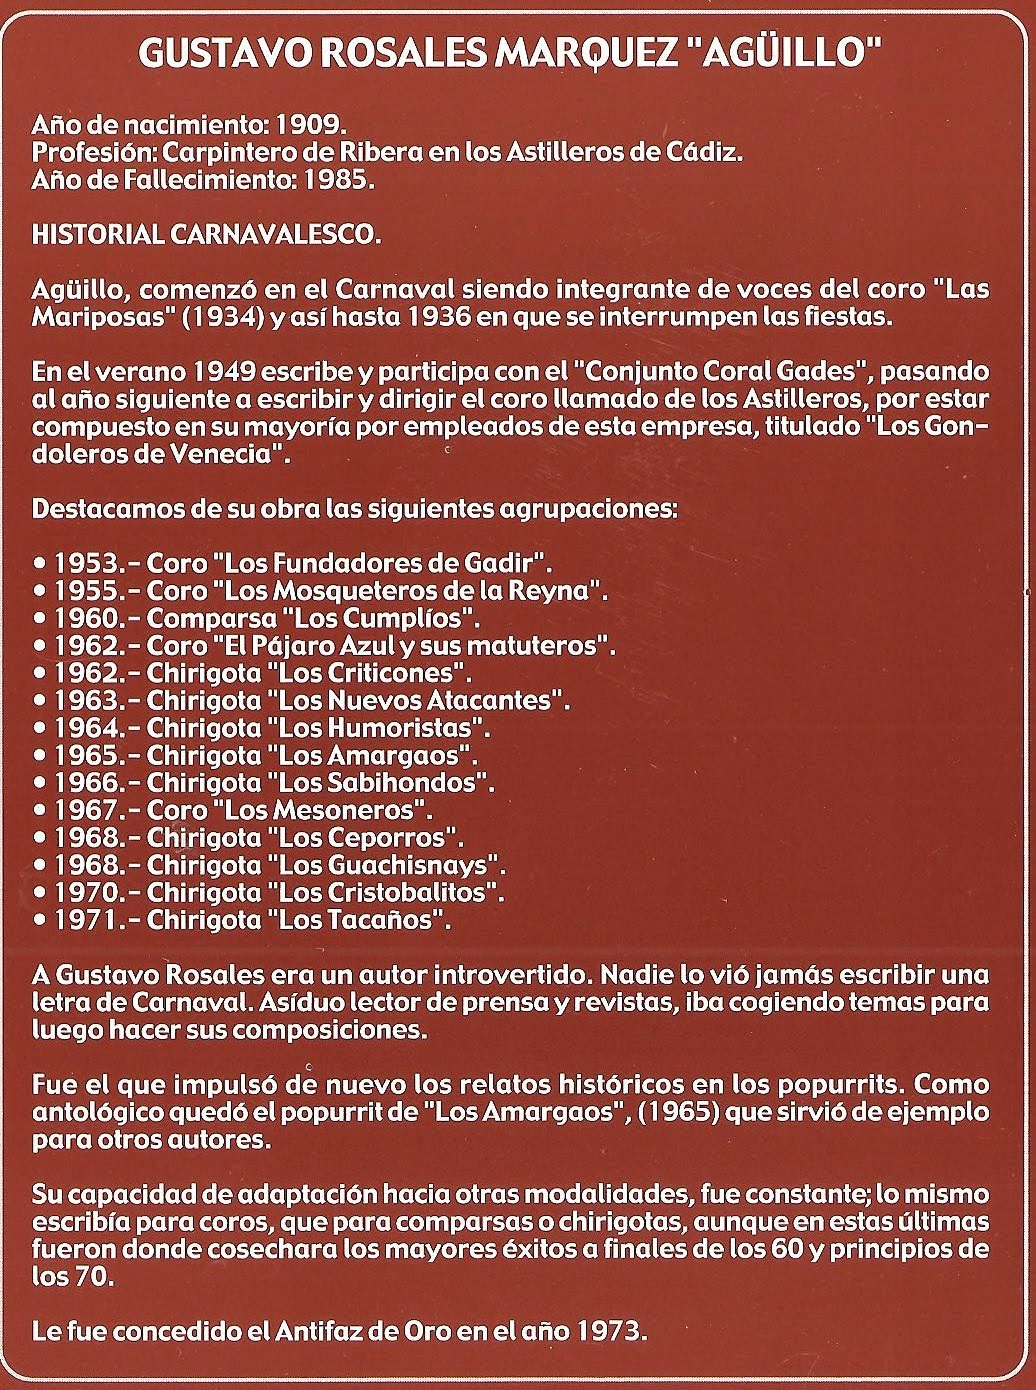
\includegraphics[width=\textwidth,height=4cm,keepaspectratio]{imgs/popurri13.jpg}
        \caption{popurri13}
    \end{subfigure}
    \hfill
    \begin{subfigure}[b]{0.31\textwidth}
        \centering
        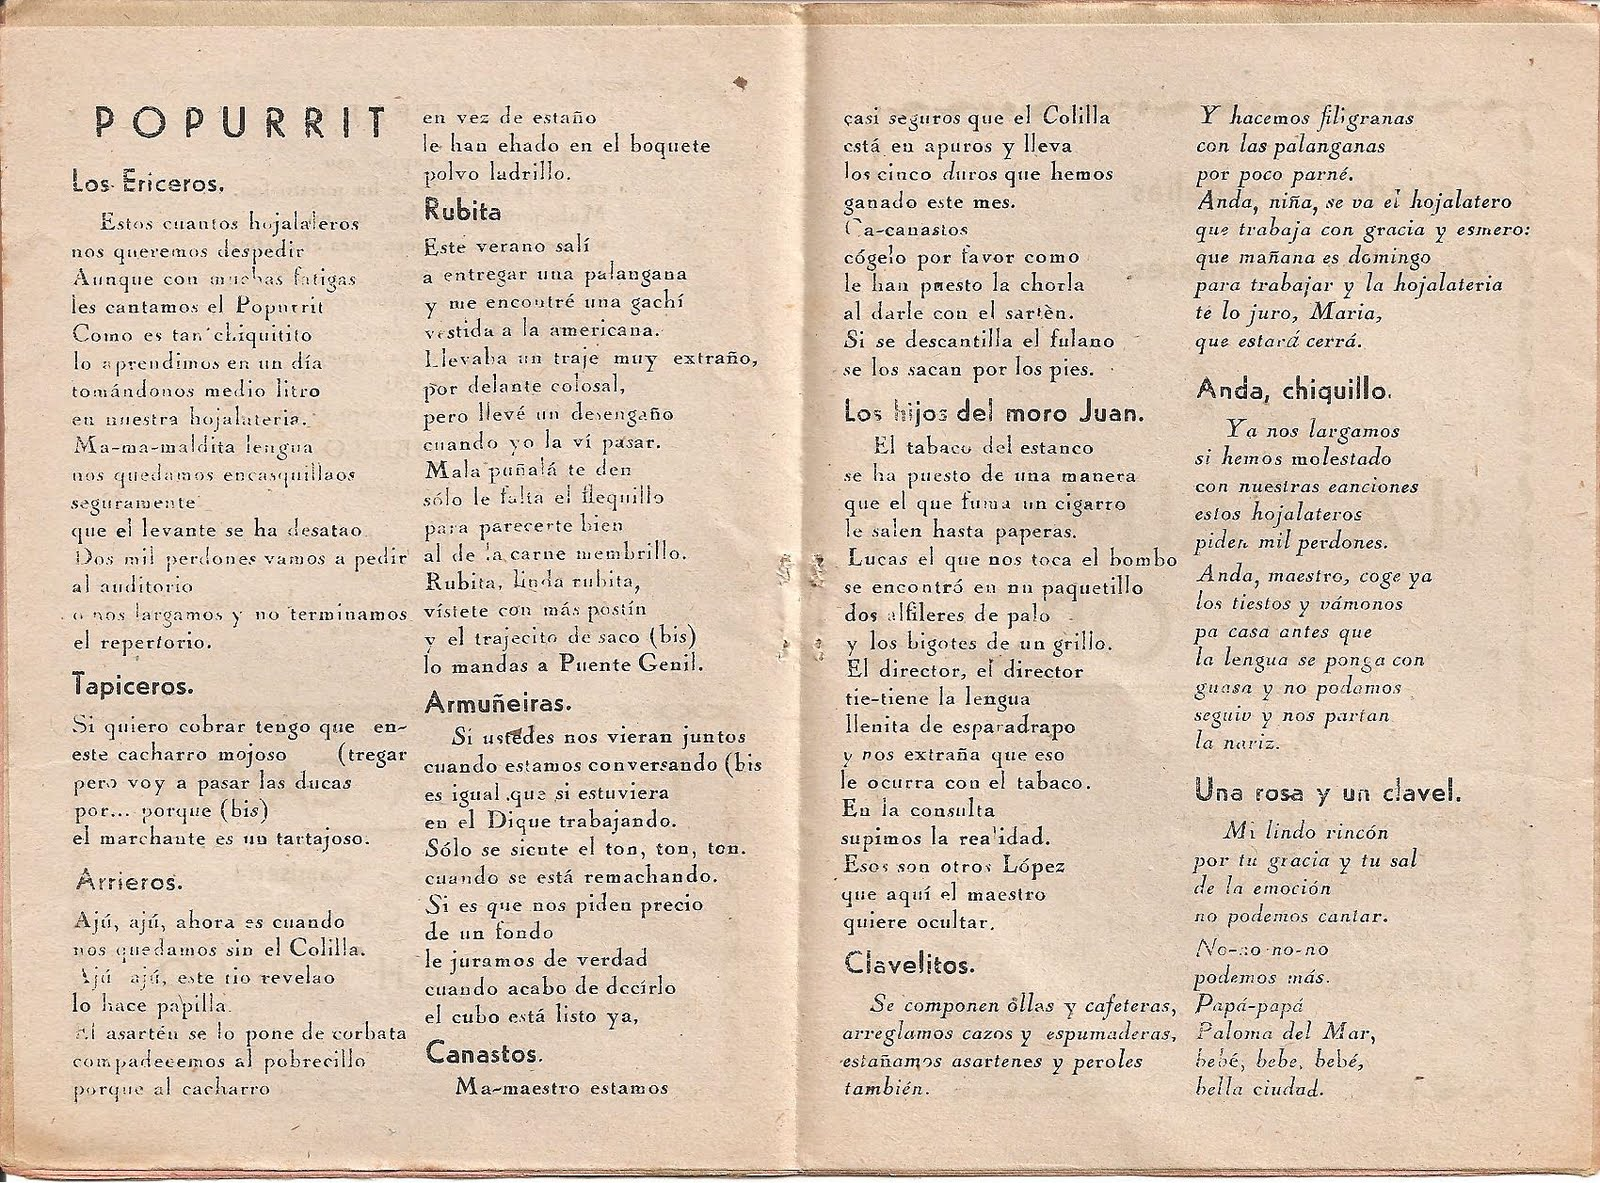
\includegraphics[width=\textwidth,height=4cm,keepaspectratio]{imgs/popurri14.jpg}
        \caption{popurri14}
    \end{subfigure}
    \hfill
    \begin{subfigure}[b]{0.31\textwidth}
        \centering
        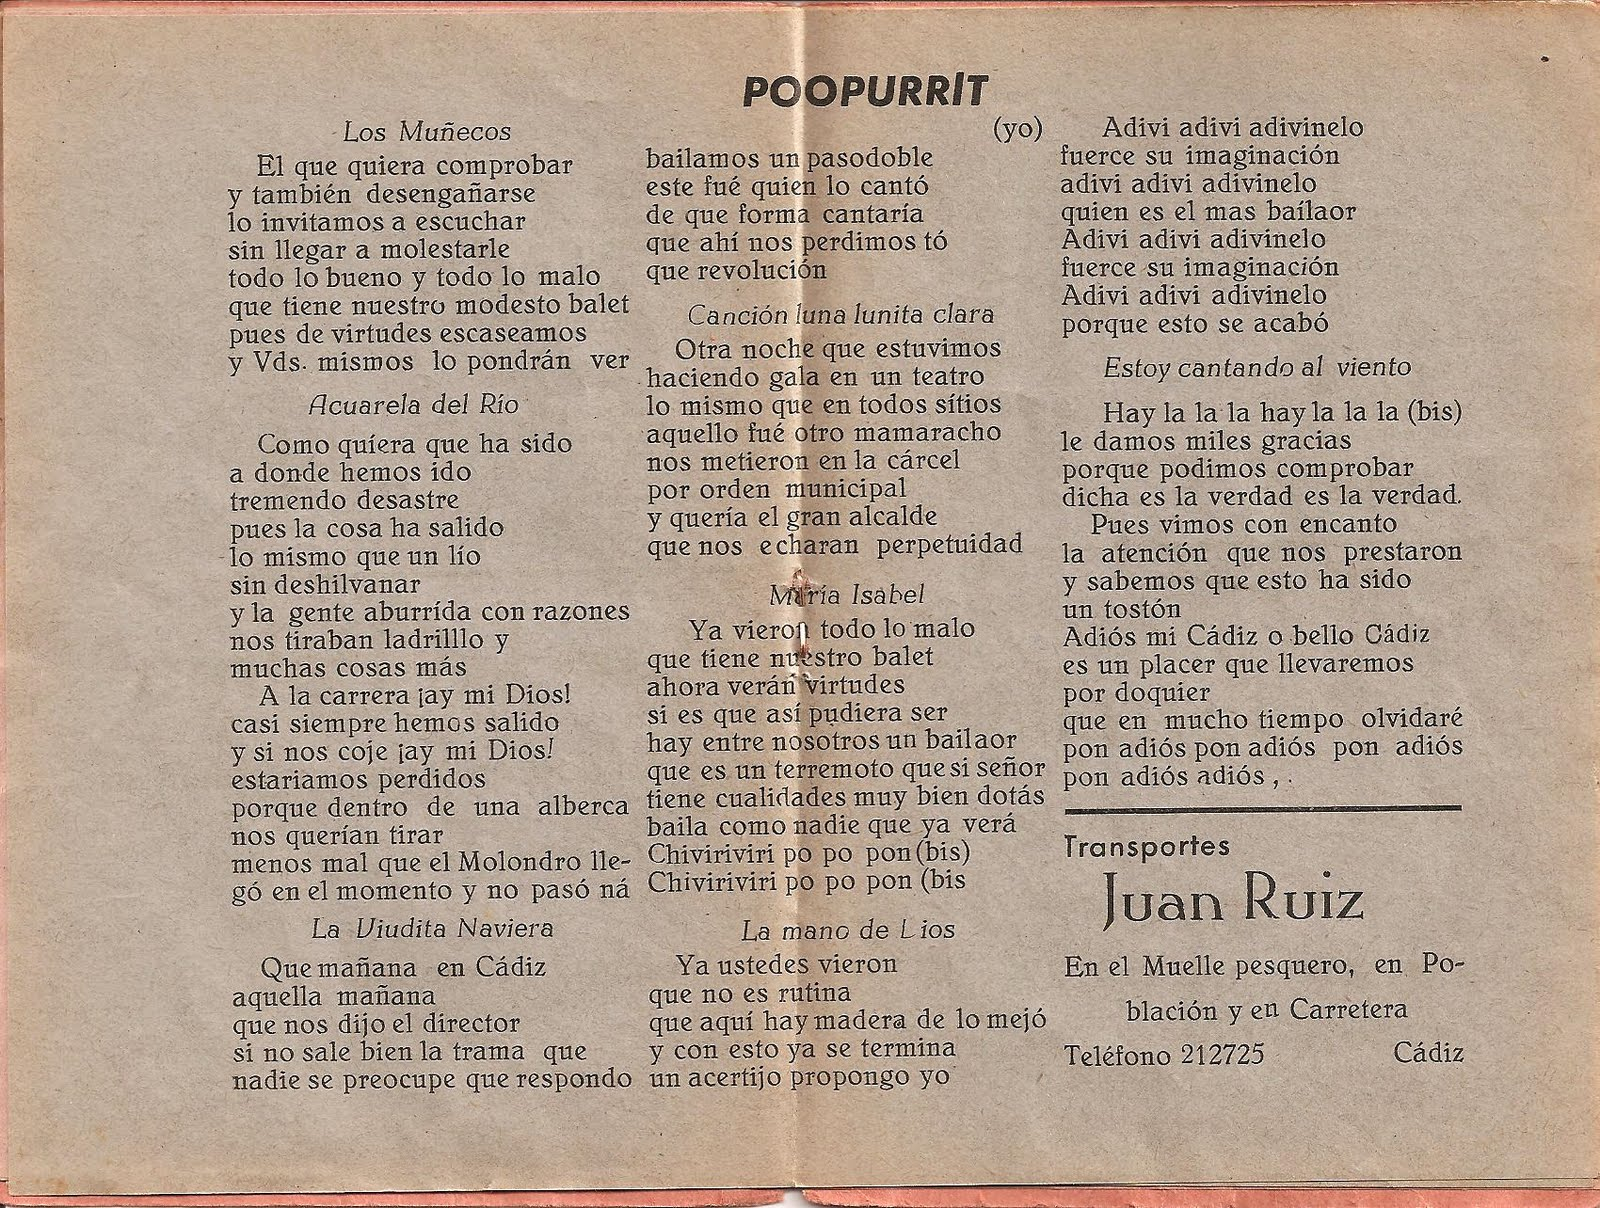
\includegraphics[width=\textwidth,height=4cm,keepaspectratio]{imgs/popurri15.jpg}
        \caption{popurri15}
    \end{subfigure}

    \vspace{0.4cm}

    \begin{subfigure}[b]{0.31\textwidth}
        \centering
        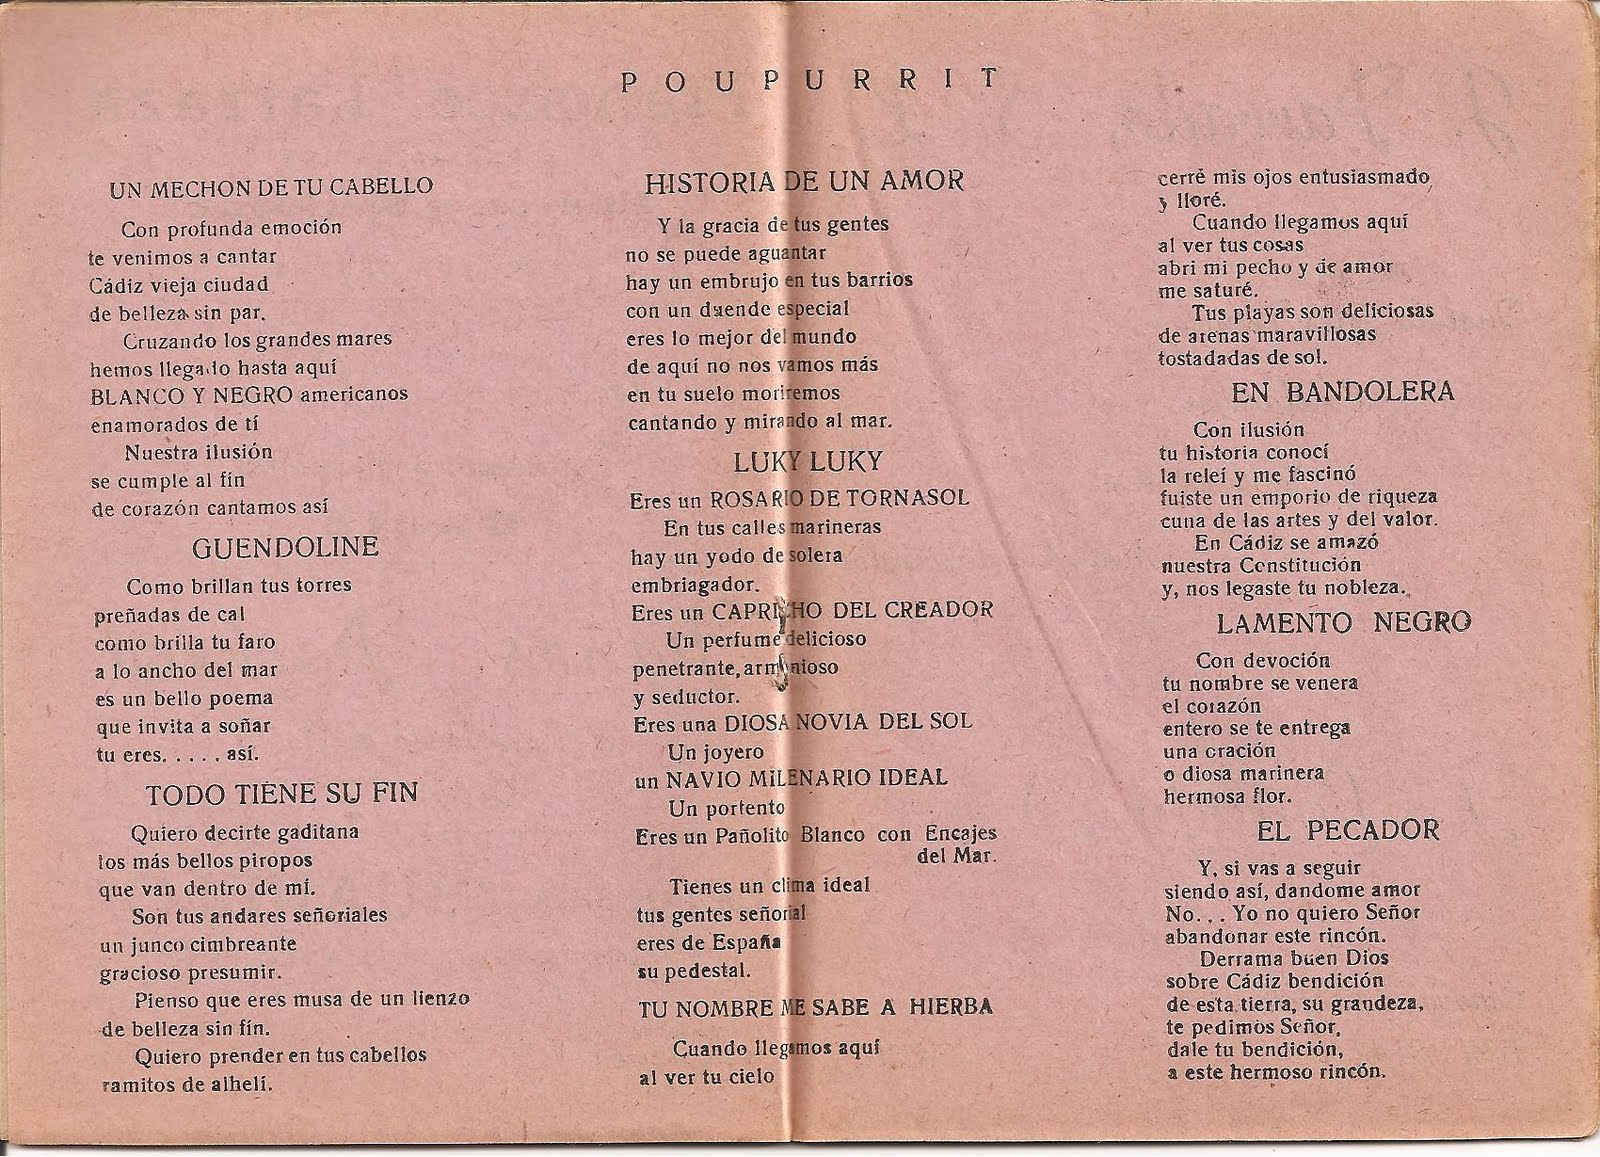
\includegraphics[width=\textwidth,height=4cm,keepaspectratio]{imgs/popurri16.jpg}
        \caption{popurri16}
    \end{subfigure}
    \hfill
    \begin{subfigure}[b]{0.31\textwidth}
        \centering
        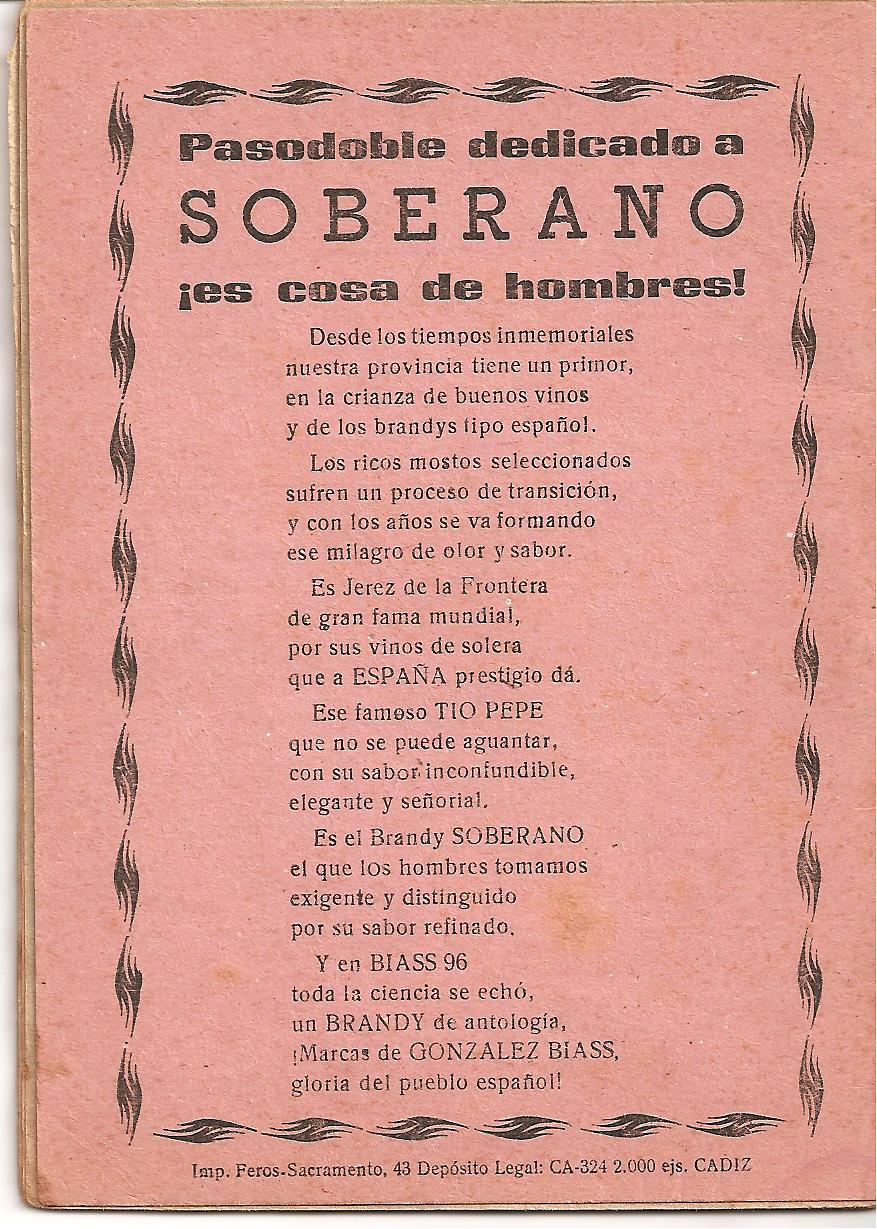
\includegraphics[width=\textwidth,height=4cm,keepaspectratio]{imgs/popurri17.jpg}
        \caption{popurri17}
    \end{subfigure}
    \hfill
    \begin{subfigure}[b]{0.31\textwidth}
        \centering
        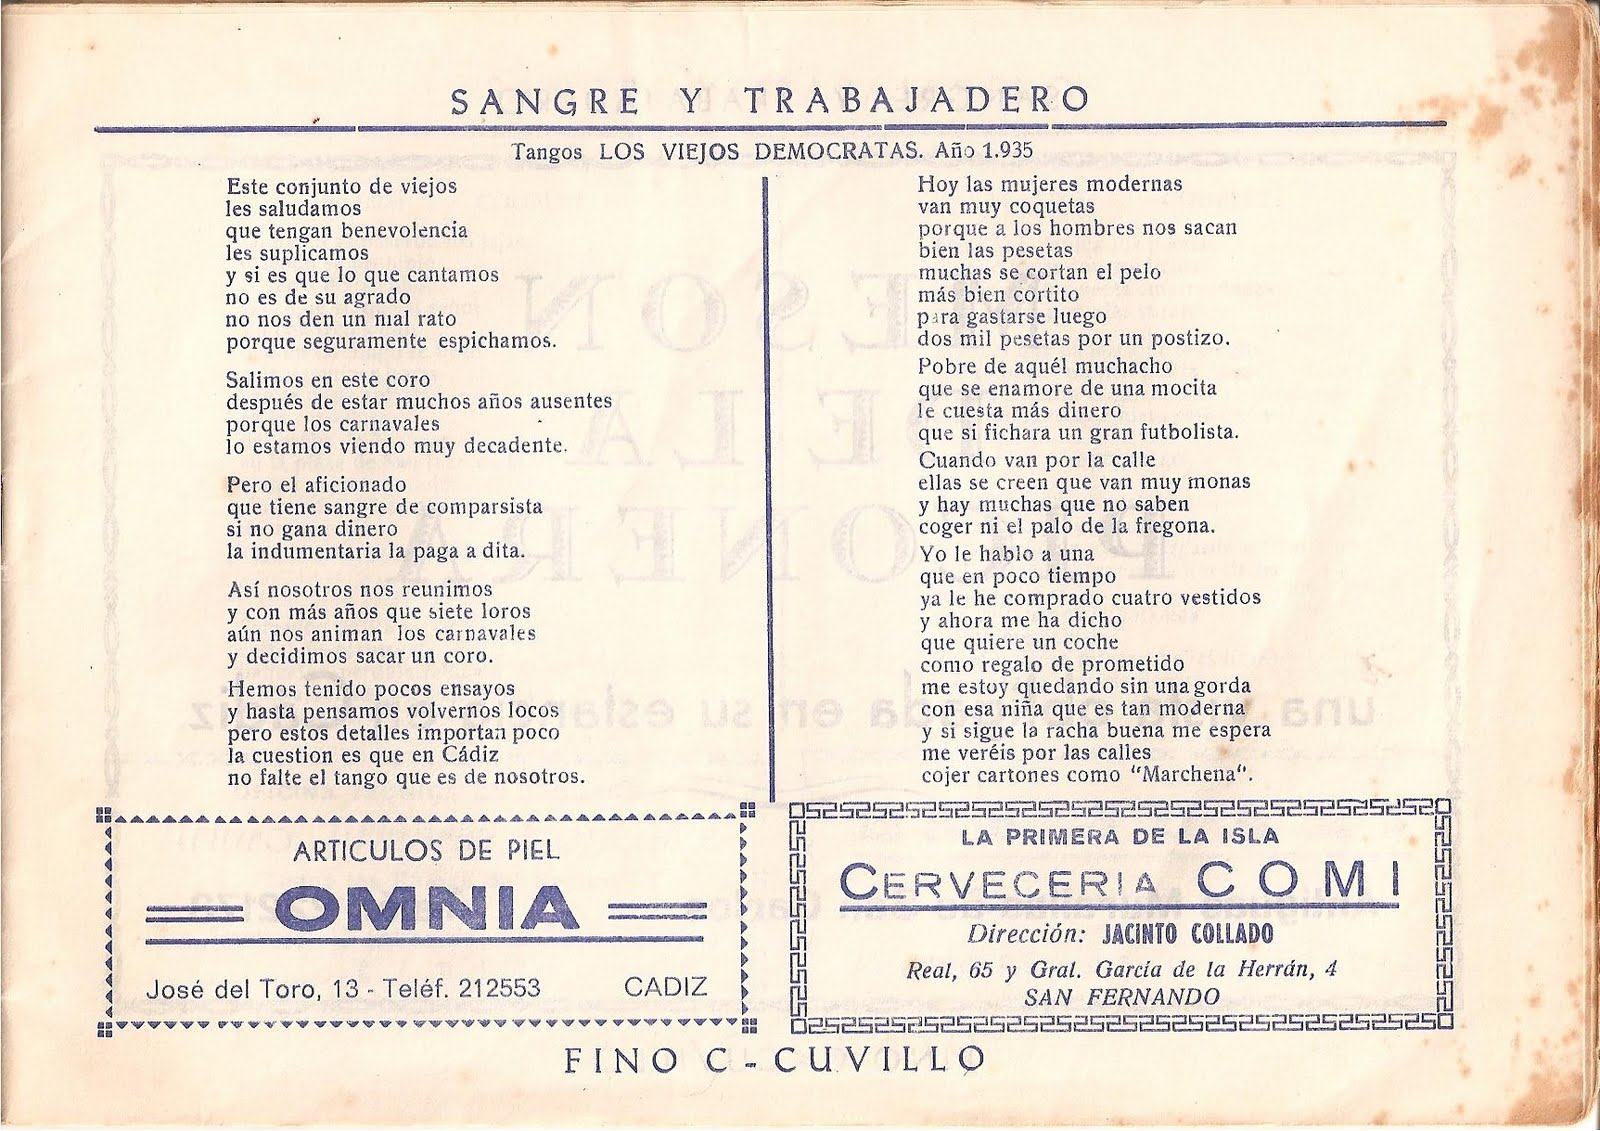
\includegraphics[width=\textwidth,height=4cm,keepaspectratio]{imgs/popurri18.jpg}
        \caption{popurri18}
    \end{subfigure}
    \caption{Galer\'ia del dataset, bloque 3 de 3.}
\end{figure}

\begin{longtable}{p{2.9cm} p{9.6cm}}
\caption{Inventario del conjunto de im\'agenes}\label{tab:inventario_imgs}\\
\toprule
\textbf{Archivo} & \textbf{Uso dentro del proyecto} \\
\midrule
\endfirsthead
\toprule
\textbf{Archivo} & \textbf{Uso dentro del proyecto} \\
\midrule
\endhead
\texttt{popurri01.jpg} & Validaci\'on, OCR por regiones y an\'alisis de layout. \\
\texttt{popurri02.jpg} & Validaci\'on, OCR por regiones y an\'alisis de layout. \\
\texttt{popurri03.jpg} & Validaci\'on, OCR por regiones y an\'alisis de layout. \\
\texttt{popurri04.jpg} & Validaci\'on, OCR por regiones y an\'alisis de layout. \\
\texttt{popurri05.jpg} & Validaci\'on, OCR por regiones y an\'alisis de layout. \\
\texttt{popurri06.jpg} & Validaci\'on, OCR por regiones y an\'alisis de layout. \\
\texttt{popurri07.jpg} & Validaci\'on, OCR por regiones y an\'alisis de layout. \\
\texttt{popurri08.jpg} & Validaci\'on, OCR por regiones y an\'alisis de layout. \\
\texttt{popurri09.jpg} & Validaci\'on, OCR por regiones y an\'alisis de layout. \\
\texttt{popurri10.jpg} & Validaci\'on, OCR por regiones y an\'alisis de layout. \\
\texttt{popurri11.jpg} & Validaci\'on, OCR por regiones y an\'alisis de layout. \\
\texttt{popurri12.jpg} & Validaci\'on, OCR por regiones y an\'alisis de layout. \\
\texttt{popurri13.jpg} & Validaci\'on, OCR por regiones y an\'alisis de layout. \\
\texttt{popurri14.jpg} & Validaci\'on, OCR por regiones y an\'alisis de layout. \\
\texttt{popurri15.jpg} & Validaci\'on, OCR por regiones y an\'alisis de layout. \\
\texttt{popurri16.jpg} & Validaci\'on, OCR por regiones y an\'alisis de layout. \\
\texttt{popurri17.jpg} & Validaci\'on, OCR por regiones y an\'alisis de layout. \\
\texttt{popurri18.jpg} & Validaci\'on, OCR por regiones y an\'alisis de layout. \\
\bottomrule
\end{longtable}

\section{Proceso de instalaci\'on del sistema}

El proyecto est\'a preparado principalmente para Windows con Python 3.11, aunque parte del
flujo tambi\'en puede adaptarse a otros entornos. La instalaci\'on recomendada se realiza
mediante el script \texttt{install.bat}, que automatiza el orden correcto de dependencias.

\subsection{Requisitos previos}

Antes de instalar los paquetes Python es necesario comprobar:

\begin{itemize}
    \item Python 3.10 o 3.11.
    \item Tesseract OCR si se quiere utilizar ese motor.
    \item Git para descargas autom\'aticas de modelos.
    \item GPU NVIDIA si se pretende usar DeepSeek y acelerar los m\'etodos de layout basados en DL.
\end{itemize}

El proyecto incluye un comprobador de prerequisitos:

\begin{lstlisting}[language=bash, caption={Verificacion inicial del entorno}]
py -3.11 check_prerequisites.py
\end{lstlisting}

\subsection{Instalaci\'on recomendada}

La instalaci\'on recomendada en Windows es:

\begin{lstlisting}[language=bash, caption={Instalacion automatica recomendada}]
install.bat
\end{lstlisting}

Este script realiza las siguientes tareas:

\begin{enumerate}
    \item Verifica Python 3.11 y Tesseract,
    \item Detecta si el equipo tiene GPU o solo CPU,
    \item Instala la versi\'on adecuada de PyTorch,
    \item Instala PaddleOCR, Docling y el resto de dependencias,
    \item Descarga el modelo de DocLayout-YOLO,
    \item Copia \texttt{sitecustomize.py} a \texttt{site-packages} para compatibilidad con DeepSeek.
\end{enumerate}

\subsection{Notas de compatibilidad importantes}

Una de las partes m\'as delicadas del proyecto ha sido la convivencia entre Docling y
DeepSeek-OCR dentro del mismo entorno Python. La configuraci\'on validada del proyecto es:

\begin{itemize}
    \item \texttt{transformers==4.53.3},
    \item \texttt{tokenizers>=0.21.0,<0.22.0},
    \item Uso de \texttt{sitecustomize.py} para reexponer s\'imbolos esperados por DeepSeek.
\end{itemize}

Tambi\'en se comprob\'o que DeepSeek funciona de forma m\'as estable sobre regiones con
tama\~no \texttt{1024 x 1024} que con \texttt{640 x 640}, donde aparecieron errores internos.

\section{Proceso de uso del sistema}

El sistema se puede utilizar por fases, desde pruebas individuales hasta evaluaci\'on completa.

\subsection{Detecci\'on de layout}

Para detectar regiones de texto en una imagen se utiliza \texttt{detect\_columns.py}.

\begin{lstlisting}[language=bash, caption={Ejemplos de deteccion de layout}]
py -3.11 detect_columns.py --image imgs/popurri01.jpg --method opencv --debug
py -3.11 detect_columns.py --image imgs/popurri01.jpg --method doclayout --debug
py -3.11 detect_columns.py --image imgs/popurri01.jpg --method yolo11 --yolo11-size nano --debug
py -3.11 detect_columns.py --image imgs/popurri01.jpg --method paddleocr --debug
py -3.11 detect_columns.py --image imgs/popurri01.jpg --method docling --debug
\end{lstlisting}

\subsection{OCR por imagen o por carpeta}

Cada motor dispone de scripts espec\'ificos de prueba. Un ejemplo sencillo con PaddleOCR es:

\begin{lstlisting}[language=bash, caption={OCR por columnas sobre una imagen o carpeta}]
py -3.11 paddle-pruebas.py imgs/popurri01.jpg --method doclayout --debug
py -3.11 paddle-pruebas.py imgs/ --method doclayout
\end{lstlisting}

\subsection{Experimentaci\'on y ranking de layout}

El proyecto incluye un grid search sistem\'atico de configuraciones de layout:

\begin{lstlisting}[language=bash, caption={Grid search y analisis de configuraciones}]
py -3.11 experiment_models.py
py -3.11 analyze_experiments.py
\end{lstlisting}

\subsection{Validaci\'on OCR multi-motor}

La validaci\'on m\'as completa se realiza con \texttt{validate\_ocr.py}, que reutiliza la misma
detecci\'on por configuraci\'on para todos los motores OCR:

\begin{lstlisting}[language=bash, caption={Validacion multi-motor OCR}]
py -3.11 validate_ocr.py --top 3 --ocr-engines easyocr,tesseract,paddle,deepseek \
  --tesseract-cmd "C:\Program Files\Tesseract-OCR\tesseract.exe" \
  --deepseek-model-path ".\models\DeepSeek-OCR"
\end{lstlisting}

\subsection{Comparaci\'on contra ground truth}

La medici\'on final de calidad se obtiene mediante:

\begin{lstlisting}[language=bash, caption={Comparacion OCR vs ground truth}]
py -3.11 compare_validation_vs_ground_truth.py
\end{lstlisting}

Las salidas m\'as importantes del proyecto quedan almacenadas en:

\begin{itemize}
    \item \texttt{validation\_results/}
    \item \texttt{experiment\_results.json}
    \item \texttt{experiment\_ranking.csv}
    \item \texttt{ocr\_gt\_comparison\_report.csv}
    \item \texttt{ocr\_gt\_comparison\_report.txt}
\end{itemize}

\section{Desarrollo experimental del proyecto}

\subsection{Fase 1: detecci\'on de layout}

La primera fase consisti\'o en validar distintos detectores de layout sobre el conjunto de
18 im\'agenes. El resultado m\'as llamativo fue que el enfoque heur\'istico con OpenCV obtuvo
una cobertura media muy superior al resto en este dataset concreto.

Esto sugiere que, para este tipo de material hist\'orico, el problema dominante no siempre es
la falta de capacidad del modelo profundo, sino la capacidad de adaptarse a estructuras muy
regulares y a textos impresos grandes sobre fondos relativamente claros.

\subsection{Fase 2: grid search}

El grid search recorri\'o las combinaciones de:

\begin{itemize}
    \item Familias \texttt{doclayout} y \texttt{yolo11}: \texttt{conf x nms\_iou x merge\_distance},
    \item Familias \texttt{paddleocr} y \texttt{docling}: \texttt{nms\_iou x merge\_distance},
    \item M\'etodo \texttt{opencv}: \texttt{merge\_distance}.
\end{itemize}

En total se evaluaron \textbf{164 configuraciones} de layout.

\subsection{Fase 3: ranking heur\'istico}

El ranking de configuraciones utiliza una f\'ormula basada en cobertura textual y penalizaci\'on
de solapamientos, cajas vac\'ias, cajas diminutas y duplicados. El mejor resultado global fue
OpenCV, con una cobertura media cercana al 99\% y tiempo medio de detecci\'on alrededor de 23 ms.

\begin{table}[H]
\centering
\caption{Top 10 global del ranking de configuraciones de layout}
\small
\begin{tabular}{c l c c c c c c}
\toprule
\textbf{Rank} & \textbf{M\'etodo} & \textbf{conf} & \textbf{NMS} & \textbf{Merge} & \textbf{Cobertura} & \textbf{Tiempo ms} & \textbf{Score} \\
\midrule
1 & opencv & N/A & N/A & 15 & 0.99 & 23.04 & 99.30 \\
2 & opencv & N/A & N/A & 20 & 0.99 & 23.53 & 99.30 \\
3 & opencv & N/A & N/A & 10 & 0.99 & 25.39 & 99.30 \\
4 & opencv & N/A & N/A & 5  & 0.99 & 24.13 & 99.30 \\
5 & docling & N/A & 0.50 & 20 & 0.58 & 44901.34 & 54.69 \\
6 & docling & N/A & 0.40 & 20 & 0.58 & 42212.19 & 54.69 \\
7 & docling & N/A & 0.30 & 20 & 0.58 & 44027.30 & 54.69 \\
8 & docling & N/A & 0.60 & 20 & 0.58 & 58812.06 & 54.69 \\
9 & paddleocr & N/A & 0.50 & 5 & 0.55 & 2524.57 & 53.45 \\
10 & paddleocr & N/A & 0.40 & 5 & 0.55 & 2897.68 & 53.45 \\
\bottomrule
\end{tabular}
\normalsize
\end{table}

\begin{table}[H]
\centering
\caption{Campos utilizados en las tablas de ranking de layout}
\small
\begin{tabular}{p{3.2cm} p{10.3cm}}
\toprule
\textbf{Campo} & \textbf{Significado} \\
\midrule
Rank & Posici\'on de la configuraci\'on en el ranking global. \\
M\'etodo & Familia de detector utilizada para localizar regiones de texto. \\
conf & Umbral de confianza del detector cuando el m\'etodo lo soporta. \\
NMS & Umbral de Non-Maximum Suppression aplicado al postprocesado de cajas. \\
Merge & Distancia en p\'ixeles usada para fusionar cajas cercanas. \\
Cobertura & Fracci\'on media de texto visible cubierta por las cajas detectadas. \\
Tiempo ms & Tiempo medio de detecci\'on por imagen en milisegundos. \\
Score & M\'etrica heur\'istica final del ranking, derivada de cobertura y penalizaciones. \\
\bottomrule
\end{tabular}
\normalsize
\end{table}

\begin{table}[H]
\centering
\caption{Mejor configuraci\'on obtenida por cada familia de layout}
\small
\begin{tabular}{>{\raggedright\arraybackslash}p{2.1cm} >{\raggedright\arraybackslash}p{3.5cm} c c c c c}
\toprule
\textbf{M\'etodo} & \textbf{Configuraci\'on} & \textbf{Cobertura} & \textbf{Solap.} & \textbf{Dups} & \textbf{Tiempo ms} & \textbf{Score} \\
\midrule
OpenCV & mg=15 & 0.99 & 0.00 & 0.00 & 23.04 & 99.30 \\
Docling & nms=0.50, mg=20 & 0.58 & 0.08 & 0.00 & 44901.34 & 54.69 \\
PaddleOCR & nms=0.50, mg=5 & 0.55 & 0.02 & 0.00 & 2524.57 & 53.45 \\
DocLayout & conf=0.10, nms=0.30, mg=5 & 0.56 & 0.08 & 0.06 & 15881.93 & 52.72 \\
YOLO11 & conf=0.10, nms=0.30, mg=20 & 0.12 & 0.01 & 0.00 & --- & 11.22 \\
\bottomrule
\end{tabular}
\normalsize
\end{table}

\begin{table}[H]
\centering
\caption{Campos utilizados en la comparativa por familia de layout}
\small
\begin{tabular}{p{3.2cm} p{10.3cm}}
\toprule
\textbf{Campo} & \textbf{Significado} \\
\midrule
Cobertura & Proporci\'on media de texto recuperado por las cajas detectadas. \\
Solap. & Solapamiento medio entre cajas; valores altos suelen indicar redundancia. \\
Dups & Duplicados medios detectados tras el postprocesado. \\
Tiempo ms & Tiempo medio de detecci\'on por imagen. \\
Score & Puntuaci\'on final del ranking heur\'istico. \\
\bottomrule
\end{tabular}
\normalsize
\end{table}

La tabla anterior resume una conclusi\'on importante del proyecto: en este dataset concreto,
OpenCV supera con mucha claridad a los m\'etodos basados en modelos profundos en cobertura y
coste computacional. Docling y PaddleOCR se comportan de forma razonable, mientras que YOLO11
queda claramente por debajo.

\subsection{Fase 4: validaci\'on OCR multi-motor}

Una vez seleccionadas las configuraciones m\'as prometedoras, se ejecut\'o OCR con varios motores
sobre las mismas regiones detectadas. Esto elimina el sesgo que se producir\'ia si cada OCR
trabajara sobre segmentaciones distintas.

La comparativa final frente a ground truth mostr\'o que la mejor combinaci\'on fue:

\begin{center}
\textbf{OpenCV + DeepSeek-OCR}
\end{center}

con una \textbf{accuracy de contenido del 95.35\%}.

\begin{table}[H]
\centering
\caption{Comparativa de motores OCR sobre la mejor familia de layout (OpenCV)}
\small
\begin{tabular}{>{\raggedright\arraybackslash}p{2.4cm} >{\centering\arraybackslash}p{1.7cm} >{\centering\arraybackslash}p{1.7cm} >{\centering\arraybackslash}p{2.1cm} >{\centering\arraybackslash}p{2.0cm} >{\centering\arraybackslash}p{2.0cm}}
\toprule
\textbf{Motor OCR} & \textbf{CER contenido} & \textbf{WER contenido} & \textbf{Acc. contenido} & \textbf{Reorder ratio} & \textbf{Tiempo ms/img} \\
\midrule
DeepSeek & 0.0383 & 0.0588 & 95.35\% & 0.1667 & 65304.02 \\
PaddleOCR & 0.0517 & 0.0662 & 94.25\% & 0.2222 & 10446.79 \\
Tesseract & 0.0745 & 0.1048 & 91.34\% & 0.2778 & 1691.77 \\
EasyOCR & 0.0970 & 0.1439 & 88.43\% & 0.5000 & 17594.06 \\
\bottomrule
\end{tabular}
\normalsize
\end{table}

Esta tabla deja ver el principal compromiso del sistema:

\begin{itemize}
    \item DeepSeek obtiene la mayor calidad, pero es con diferencia el m\'as costoso en tiempo.
    \item Tesseract es mucho m\'as r\'apido y mantiene una calidad bastante competitiva.
    \item PaddleOCR queda muy equilibrado entre calidad y coste.
    \item EasyOCR fue el menos preciso de los cuatro en este escenario.
\end{itemize}

\begin{table}[H]
\centering
\caption{Mejor resultado encontrado por familia de layout usando OCR DeepSeek}
\small
\begin{tabular}{>{\raggedright\arraybackslash}p{3.1cm} >{\centering\arraybackslash}p{1.5cm} >{\centering\arraybackslash}p{1.5cm} >{\centering\arraybackslash}p{2.0cm} >{\centering\arraybackslash}p{1.8cm} >{\centering\arraybackslash}p{2.0cm}}
\toprule
\textbf{Layout} & \textbf{CER cont.} & \textbf{WER cont.} & \textbf{Acc. contenido} & \textbf{Disorder} & \textbf{Tiempo ms/img} \\
\midrule
OpenCV mg10 & 0.0383 & 0.0588 & 95.35\% & 0.0353 & 65304.02 \\
PaddleOCR nms0.30 mg5 & 0.1614 & 0.1875 & 82.82\% & 0.2429 & 116919.61 \\
Docling nms0.30 mg20 & 0.2135 & 0.2423 & 77.50\% & 0.0986 & 92417.13 \\
\bottomrule
\end{tabular}
\normalsize
\end{table}

\scriptsize
\begin{longtable}{>{\raggedright\arraybackslash}p{4.1cm} >{\centering\arraybackslash}p{1.5cm} >{\centering\arraybackslash}p{1.4cm} >{\centering\arraybackslash}p{1.4cm} >{\centering\arraybackslash}p{1.6cm} >{\centering\arraybackslash}p{1.8cm}}
\caption{Top 20 combinaciones OCR-layout por accuracy de contenido}\label{tab:top20_ocr_layout}\\
\toprule
\textbf{Layout} & \textbf{OCR} & \textbf{CER cont.} & \textbf{WER cont.} & \textbf{Acc. cont.} & \textbf{Tiempo ms/img} \\
\midrule
\endfirsthead
\toprule
\textbf{Layout} & \textbf{OCR} & \textbf{CER cont.} & \textbf{WER cont.} & \textbf{Acc. cont.} & \textbf{Tiempo ms/img} \\
\midrule
\endhead
OpenCV mg10 & deepseek & 0.0383 & 0.0588 & 95.35\% & 65304.02 \\
OpenCV mg15 & deepseek & 0.0383 & 0.0588 & 95.35\% & 67195.96 \\
OpenCV mg20 & deepseek & 0.0383 & 0.0588 & 95.35\% & 64783.07 \\
OpenCV mg5 & deepseek & 0.0383 & 0.0588 & 95.35\% & 64955.83 \\
OpenCV mg10 & paddle & 0.0517 & 0.0662 & 94.25\% & 10446.79 \\
OpenCV mg15 & paddle & 0.0517 & 0.0662 & 94.25\% & 10391.83 \\
OpenCV mg20 & paddle & 0.0517 & 0.0662 & 94.25\% & 10654.37 \\
OpenCV mg5 & paddle & 0.0517 & 0.0662 & 94.25\% & 10588.87 \\
OpenCV mg10 & tesseract & 0.0745 & 0.1048 & 91.34\% & 1691.77 \\
OpenCV mg15 & tesseract & 0.0745 & 0.1048 & 91.34\% & 1743.20 \\
OpenCV mg20 & tesseract & 0.0745 & 0.1048 & 91.34\% & 1700.61 \\
OpenCV mg5 & tesseract & 0.0745 & 0.1048 & 91.34\% & 1698.91 \\
OpenCV mg10 & easyocr & 0.0970 & 0.1439 & 88.43\% & 17594.06 \\
OpenCV mg15 & easyocr & 0.0970 & 0.1439 & 88.43\% & 20446.01 \\
OpenCV mg20 & easyocr & 0.0970 & 0.1439 & 88.43\% & 18375.31 \\
OpenCV mg5 & easyocr & 0.0970 & 0.1439 & 88.43\% & 18179.83 \\
PaddleOCR nms0.30 mg5 & deepseek & 0.1614 & 0.1875 & 82.82\% & 116919.61 \\
PaddleOCR nms0.40 mg5 & deepseek & 0.1614 & 0.1875 & 82.82\% & 96239.21 \\
PaddleOCR nms0.30 mg5 & tesseract & 0.1793 & 0.2123 & 80.75\% & 6458.41 \\
PaddleOCR nms0.40 mg5 & tesseract & 0.1793 & 0.2123 & 80.75\% & 6732.35 \\
\bottomrule
\end{longtable}
\normalsize

\scriptsize
\begin{longtable}{>{\raggedright\arraybackslash}p{4.1cm} >{\centering\arraybackslash}p{1.5cm} >{\centering\arraybackslash}p{1.4cm} >{\centering\arraybackslash}p{1.4cm} >{\centering\arraybackslash}p{1.6cm} >{\centering\arraybackslash}p{1.8cm}}
\caption{Tabla complementaria: Top 20 combinaciones OCR-layout por velocidad}\label{tab:top20_ocr_layout_rapidas}\\
\toprule
\textbf{Layout} & \textbf{OCR} & \textbf{CER cont.} & \textbf{WER cont.} & \textbf{Acc. cont.} & \textbf{Tiempo ms/img} \\
\midrule
\endfirsthead
\toprule
\textbf{Layout} & \textbf{OCR} & \textbf{CER cont.} & \textbf{WER cont.} & \textbf{Acc. cont.} & \textbf{Tiempo ms/img} \\
\midrule
\endhead
OpenCV mg10 & tesseract & 0.0745 & 0.1048 & 91.34\% & 1691.77 \\
OpenCV mg5 & tesseract & 0.0745 & 0.1048 & 91.34\% & 1698.91 \\
OpenCV mg20 & tesseract & 0.0745 & 0.1048 & 91.34\% & 1700.61 \\
OpenCV mg15 & tesseract & 0.0745 & 0.1048 & 91.34\% & 1743.20 \\
PaddleOCR nms0.30 mg5 & tesseract & 0.1793 & 0.2123 & 80.75\% & 6458.41 \\
PaddleOCR nms0.40 mg5 & tesseract & 0.1793 & 0.2123 & 80.75\% & 6732.35 \\
Docling nms0.40 mg20 & tesseract & 0.2130 & 0.2427 & 77.51\% & 9111.95 \\
Docling nms0.30 mg20 & tesseract & 0.2130 & 0.2427 & 77.51\% & 9604.09 \\
Docling nms0.50 mg20 & tesseract & 0.2130 & 0.2427 & 77.51\% & 9635.78 \\
Docling nms0.60 mg20 & tesseract & 0.2235 & 0.2541 & 76.43\% & 10362.04 \\
OpenCV mg15 & paddle & 0.0517 & 0.0662 & 94.25\% & 10391.83 \\
OpenCV mg10 & paddle & 0.0517 & 0.0662 & 94.25\% & 10446.79 \\
OpenCV mg5 & paddle & 0.0517 & 0.0662 & 94.25\% & 10588.87 \\
OpenCV mg20 & paddle & 0.0517 & 0.0662 & 94.25\% & 10654.37 \\
PaddleOCR nms0.30 mg5 & easyocr & 0.2016 & 0.2525 & 77.80\% & 15629.34 \\
PaddleOCR nms0.40 mg5 & easyocr & 0.2016 & 0.2525 & 77.80\% & 15641.97 \\
OpenCV mg10 & easyocr & 0.0970 & 0.1439 & 88.43\% & 17594.06 \\
OpenCV mg5 & easyocr & 0.0970 & 0.1439 & 88.43\% & 18179.83 \\
OpenCV mg20 & easyocr & 0.0970 & 0.1439 & 88.43\% & 18375.31 \\
OpenCV mg15 & easyocr & 0.0970 & 0.1439 & 88.43\% & 20446.01 \\
\bottomrule
\end{longtable}
\normalsize

\begin{table}[H]
\centering
\caption{Campos utilizados en las tablas OCR y de comparaci\'on con ground truth}
\small
\begin{tabular}{p{3.4cm} p{10.1cm}}
\toprule
\textbf{Campo} & \textbf{Significado} \\
\midrule
Layout & Configuraci\'on de detecci\'on usada antes del OCR. \\
OCR & Motor de reconocimiento aplicado sobre las regiones detectadas. \\
CER cont. & Error de caracteres medido sobre contenido, reduciendo el impacto del orden de lectura. \\
WER cont. & Error de palabras medido sobre contenido. \\
Acc. cont. & Accuracy agregada derivada de CER y WER de contenido. \\
Disorder & Medida de desorden respecto al ground truth; cuanto menor, mejor. \\
Reorder ratio & Proporci\'on de im\'agenes que necesitar\'ian reordenaci\'on posterior. \\
Tiempo ms/img & Tiempo medio por imagen, sumando detecci\'on y OCR. \\
\bottomrule
\end{tabular}
\normalsize
\end{table}

Esta segunda comparativa muestra que la elecci\'on del layout influye tanto como el propio OCR.
Incluso usando el mismo motor DeepSeek, la calidad cae de forma notable cuando la detecci\'on de
regiones es peor o introduce mayor fragmentaci\'on del contenido.

\subsection{Fase 5 y 6: ground truth y evaluaci\'on objetiva}

El proyecto incluye \texttt{ground\_truth/ocr\_ground\_truth.json}, que permite medir calidad real
mediante:

\begin{itemize}
    \item \textbf{CER raw}: Error a nivel de car\'acter incluyendo orden de lectura.
    \item \textbf{WER raw}: Error a nivel de palabra incluyendo orden.
    \item \textbf{CER content}: Error a nivel de contenido, con menor sensibilidad al orden.
    \item \textbf{WER content}: Equivalente a nivel de palabra.
    \item \textbf{content accuracy}: Medida resumida en escala 0--1.
    \item \textbf{disorder}: Grado de desorden respecto al ground truth.
\end{itemize}

La disponibilidad de estas m\'etricas es una de las fortalezas principales del trabajo, porque
permite distinguir entre un OCR que falla en reconocimiento y un OCR que recupera bien el texto
pero con un orden de ensamblado mejorable.

\section{Discusi\'on de resultados}

Los resultados obtenidos permiten extraer varias conclusiones t\'ecnicas relevantes:

\begin{enumerate}
    \item \textbf{El layout domina el rendimiento global.} El mejor OCR no puede compensar del todo
    una segmentaci\'on mediocre.
    \item \textbf{OpenCV funcion\'o sorprendentemente bien} en este conjunto concreto, probablemente
    porque muchas im\'agenes presentan columnas relativamente bien separadas y estructuras de texto
    amplias.
    \item \textbf{DeepSeek-OCR fue el motor m\'as preciso}, pero tambi\'en el m\'as caro en tiempo.
    \item \textbf{Tesseract sigue siendo una base muy competitiva} cuando interesa coste bajo y
    buen rendimiento general.
    \item \textbf{YOLO11 no se adapt\'o bien al dataset} y qued\'o muy lejos del resto en cobertura.
\end{enumerate}

\section{Conclusiones}

El proyecto ha terminado convertido en una plataforma de evaluaci\'on OCR bastante completa,
no solo en un conjunto de scripts aislados. Sus aportaciones principales son:

\begin{itemize}
    \item Un pipeline reproducible desde instalaci\'on hasta evaluaci\'on final,
    \item Un conjunto de 18 im\'agenes hist\'oricas con ground truth asociado,
    \item Una comparativa objetiva de varios m\'etodos de layout,
    \item Una comparativa objetiva de varios motores OCR,
    \item Resultados medibles con m\'etricas robustas.
\end{itemize}

La mejor combinaci\'on final encontrada en el proyecto ha sido \textbf{OpenCV + DeepSeek-OCR},
que alcanz\'o una accuracy de contenido del 95.35\%. Sin embargo, si se prioriza velocidad,
\textbf{OpenCV + Tesseract} ofrece un compromiso muy razonable. Por tanto, la elecci\'on \'optima
depende del objetivo operativo final:

\begin{itemize}
    \item M\'axima calidad: OpenCV + DeepSeek,
    \item Equilibrio calidad/tiempo: OpenCV + PaddleOCR,
    \item M\'inimo coste temporal: OpenCV + Tesseract.
\end{itemize}

Como trabajo futuro, los pasos m\'as naturales son mejorar la reordenaci\'on de lectura entre
regiones, ampliar el ground truth a otros tipos documentales y estudiar estrategias h\'ibridas
que usen diferentes layouts seg\'un la morfolog\'ia de la p\'agina.

\begin{thebibliography}{1}

\bibitem{tesseract}
Tesseract OCR. \url{https://github.com/tesseract-ocr/tesseract}

\bibitem{paddleocr}
PaddleOCR. \url{https://github.com/PaddlePaddle/PaddleOCR}

\bibitem{easyocr}
EasyOCR. \url{https://github.com/JaidedAI/EasyOCR}

\bibitem{docling}
IBM Docling. \url{https://github.com/docling-project/docling}

\bibitem{ultralytics}
Ultralytics YOLO. \url{https://github.com/ultralytics/ultralytics}

\end{thebibliography}

\end{document}